\documentclass[oneside, 12pt, openany]{book}

% Fonts
\usepackage[sfdefault]{atkinson} % For using a Atkinson Hyperlegible font
\usepackage[T1]{fontenc}

\usepackage[english]{babel} % English writing
\usepackage[utf8]{inputenc} % UTF8 encoding

\usepackage{graphicx} % Graphics and images
\graphicspath{ {img/} } % Images route

\usepackage[a4paper,top=30mm,left=30mm,right=25mm,bottom=35mm,headheight=55mm, footskip=20mm]{geometry} % Margin configuration

% Format packages
\usepackage{titlesec}
\usepackage{setspace}
\usepackage{ragged2e}
\usepackage{fancyhdr}
\usepackage{lastpage}
\usepackage{stackengine}
\usepackage{array}
\usepackage{url}
\usepackage{float}
\usepackage{multirow}
\usepackage{lastpage}
\usepackage{lscape}

% Links and references
\usepackage{hyperref}
\setcounter{tocdepth}{4} % Depth of the table of contents

\hypersetup
{
    bookmarksnumbered,
    breaklinks=false,
    linktocpage=false,
    colorlinks=true,
    linkcolor=black,
    citecolor=black,
    urlcolor=black,
    menucolor=black
}

% Color package
\usepackage[table,xcdraw,dvipsnames]{xcolor}

% Include pages from another PDF
\usepackage{pdfpages}

% Text generation package
\usepackage{lipsum}

% Table generator package
\usepackage{tabularx}

% List management package
\usepackage{enumitem}

% Captions package
\usepackage{caption} 
\captionsetup[table]{skip=10pt}

% Quotes packages
\usepackage{csquotes}
\usepackage{epigraph}

% Math packages
\usepackage{amsmath}

% Loads the configuration tex file
\setcounter{secnumdepth}{4} % For numbering subsubsections

% Section names format
\titleformat{\chapter}[block]
{\normalfont\Huge\bfseries\singlespacing}{\thechapter}{1em}{\Huge}
\titlespacing*{\chapter}{0pt}{-62pt}{0pt}

\titleformat{\section}[block]
{\normalfont\large\bfseries}{\thesection}{4pt}{\large}
\titlespacing*{\section}{0pt}{\baselineskip}{0pt}

\titleformat{\subsection}[block]
{\normalfont\normalsize\bfseries}{\thesubsection}{4pt}{\normalsize}
\titlespacing*{\subsection}{0pt}{0pt}{0pt}

\titleformat{\subsubsection}[block]
{\normalfont\normalsize\bfseries}{\thesubsubsection}{4pt}{\normalsize}
\titlespacing*{\subsubsection}{0pt}{0pt}{0pt}


% Header and footer format
\fancyhf{} % Clear every field

\fancyhead[L]{\bfseries{\large TODO: uniovi img}}
\fancyhead[C]{\bfseries{\large \documentname}}
\fancyhead[R]{\bfseries{\large TODO: eii img}}

\fancyfoot[CE,CO,LE,LO,RE,RO]{} % Clear all footers
\fancyfoot[C]
{
    \begin{tabular}{|ll|c}
        \hline
        \multicolumn{3}{|l|}{\tfg} \\ 
        \hline
        \textbf{Author:} Hugo Fonseca Díaz & & 
        \multicolumn{1}{c|}{
            \multirow{3}{*}
            {
                Page \thepage \hspace{1pt} of {\hypersetup{linkcolor=black} \pageref*{LastPage}}
            }
        } \\ 
        \cline{1-2}
        \textbf{Supervisors:} Raúl Mencía Cascallana, Carlos Mencía Cascallana & & \multicolumn{1}{c|}{} \\
        \cline{1-2}
        \documentdate & \version & \multicolumn{1}{c|}{} \\
        \hline
    \end{tabular}
}

\renewcommand{\headrulewidth}{0.5pt}
\renewcommand{\footrulewidth}{0pt}

% Plain rewrite for having the same header and footer in all pages
\fancypagestyle{plain}
{

    % Header and footer format
    \fancyhf{} % Clear every field

    \fancyhead[L]{\bfseries{\large TODO: uniovi img}}
    \fancyhead[C]{\bfseries{\large \documentname}}
    \fancyhead[R]{\bfseries{\large TODO: eii img}}

    \fancyfoot[CE,CO,LE,LO,RE,RO]{} % Clear all footers
    \fancyfoot[C]
    {
        \begin{tabular}{|ll|c}
            \hline
            \multicolumn{3}{|l|}{\tfg} \\ 
            \hline
            \textbf{Author:} Hugo Fonseca Díaz & & 
            \multicolumn{1}{c|}{
                \multirow{3}{*}
                {
                    Page \thepage \hspace{1pt} of {\hypersetup{linkcolor=black} \pageref*{LastPage}}
                }
            } \\ 
            \cline{1-2}
            \textbf{Supervisors:} Raúl Mencía Cascallana, Carlos Mencía Cascallana & & \multicolumn{1}{c|}{} \\
            \cline{1-2}
            \documentdate & \version & \multicolumn{1}{c|}{} \\
            \hline
        \end{tabular}
    }

    \renewcommand{\headrulewidth}{0.5pt}
    \renewcommand{\footrulewidth}{0pt}

}


\pagestyle{fancy}
\restylefloat{table}

% Captions config
\floatstyle{plaintop}
\restylefloat{table}


% Variable config
\newcommand{\documentname}{Index}
\newcommand{\version}{\textbf{Version:} 1.0}
\newcommand{\documentdate}{\textbf{Date:} Appril 16\textsuperscript{th}, 2022}
\newcommand{\tfg}{TODO: TFG Full name}
\setcounter{chapter}{-1}




% Document starts
\begin{document}


% Documentation cover page

% Front cover
\includepdf[pages=1]{other/covers.pdf}




\renewcommand{\contentsname}{\empty}
\renewcommand{\documentname}{Index}


\chapter{Index}

\begingroup
\let\clearpage\relax

\vspace{5mm}

% Index
\tableofcontents

\endgroup


\justify % Justify text
\setlength{\parskip}{\baselineskip} % Separate paragraphs by one line
\onehalfspacing


% Content block
{
    % Links in the content block appear in blue
    \hypersetup{linkcolor=blue}

    \newpage
    \renewcommand{\documentname}{Overview}

\chapter{Overview}

This document presents all the important information regarding the \textit{\tfg} end-of-degree thesis.

It is important to note that the structure of the contents for this document is done following the criteria and recommendations of the template document for Degree's and Master's Thesis of the School of Computing Engineering of Oviedo (version 1.4) \cite{doc-template} by Redondo. However, some additional chapters were introduced in order to capture the particularity of the work carried out, inspired by the research of de la Cruz \cite{metaheuristics-groups}.

\begin{description}

    \item \textbf{Report}. This is the chapter where I explain the personal motivation to take on this project, as well as give a brief explanation on the nature of the project and what it covers. 

    \item \textbf{Introduction}. Here we explain in a simple way the problem we want to solve, what reasons are behind the development of the project and give a description of the current situation of the School with regard to this and other similar problems.

    \item \textbf{Theoretical aspects}. The first chapter delving into the theory supporting the developed system. One example of an assignment problem is presented and solved using a greedy algorithm and a genetic algorithm, which helps to better internalize the concepts.

    \item \textbf{Problem definition}. Here the formulation of the problem as an assignment problem is elaborated. 

    \item \textbf{Proposed solution}. This chapter lays down in detail the proposed solution to the previously defined assignment problem by means of a genetic and greedy algorithms.

    \item \textbf{Project planning and budget overview}. For the planning, the Gantt chart of the project is shown, as well as the work breakdown structure. The internal and client budgets are presented, but not how they were calculated. That goes in the budget section.

    \item \textbf{Analysis}. An analysis of the system, with the system requirements, draft diagrams, use cases and the test plan specification. 

    \item \textbf{System design}. The technical details of the system analysed in the previous section. Here we include the finalised diagrams, as well as the arquitecture of the system and the in-depth test plan.

    \item \textbf{System implementation}. Details of the development of the software. The programming languages, standards and tools used to code the system, and all the relevant information gathered in the process of creating the system.

    \item \textbf{Test development}. A rundown of all the testing done for the system, with explanations for every test and the obtained results. 

    \item \textbf{Experimental results}. The conclusions reached after experimenting with different input data and the optimal configuration for the genetic algorithm's parameters. 

    \item \textbf{System manuals}. All the manuals for the system, with screenshots and guided steps meant to help the target audience for each document. 

    \item \textbf{Conclusions and future work}. The conclusions after the implementation of the project are given, as well as a list of possible improvements and new functionalities for the prototype. 

    \item \textbf{Budget}. Here we give the full details for the elaboration of the internal and client budgets, with all the intermediate steps that led us to that result. 

    \item \textbf{Annexes}. The glossary of definitions and abbreviations and a small commentary on the submitted files.

    \item \textbf{Source code}. The \textit{javadoc} of the software developed. 

\end{description}

 

    \newpage
    \renewcommand{\documentname}{Report}

\chapter{Report}

\section{Summary of the document}

\textbf{TODO: EXPLAIN MORE DETAILS ABOUT THE SECTIONS}

This document presents all the important information regarding the \textit{\tfg} end-of-degree thesis.

First, a report of the project is given. It functions as a general summary of the work done. This is followed by the introduction to the project, which gives a justification for the project, lays down the objectives and analyses the past and present situation.

After that, the theoretical sections of the project are presented. They consist of a number of definitions of key concepts, a formal definition of the problem to solve and a detailed explanation of the proposed solution.

Then the project planning and budget overview are shown.

Subsequent to the project planning rundown follow the software engineering chapters, which include the system analysis, design and implementation and the test development. 

After outlining the specifications of the system, the results of the experiments conducted are listed.

The system manuals for the programmer and the user are handed.

Finally, the conclusions and future work are listed, along with the final budgets, the bibliography, annexes and the source code.

It is important to note that the organization of the contents for this document is done following the criteria and recommendations of the template document for Degree's and Master's Thesis of the School of Computing Engineering of Oviedo (version 1.4) by J. M. Redondo.

\section{Purpose}

This project aims to create a program that automates the process of assigning classrooms to all the groups of a given semester.

The implementation of this system is intended to assist in the work of the supervisor for this process, and provide an efficient and flexible tool that expands the possibilities of such work.

To do so, the program executes two algorithms, a genetic algorithm guided by a greedy algorithm. For a more detailed view on these algorithms the reader might refer to \ref{alg-studies}.

Along with the system, the user and programmer manuals are submitted. These have the purpose of teaching how to use, maintain and extend the system.

\section{Standards and references}

\subsection{Standards}

\textit{UNE 157801. General criteria for the design of information systems projects.} This standard is used for defining the structure and contents of this document. However, some sections have been added, removed or modified to fit the format of a final degree project. A conclusions chapter has been introduced to the general structure as well.

\subsection{Licenses}

The software of this project is licensed under the GNU General Public License v2.0.

\subsection{Other references}

\textit{Java Code Conventions.} Set of guidelines and conventions for programmers to consider when using the Java programming language.

\section{Definitions and abbreviations}

Listed below is a glossary of definitions and abbreviations used in the document whose meaning may not be obvious.

Glossary of definitions:

\begin{itemize}
    \item \textbf{Genetic algorithm:} metaheuristic search and optimization algorithm. 
    \item \textbf{Greedy algorithm:} algorithm that builds the solution in successive steps, always trying to take the optimal solution for each step
    \item \textbf{Heuristic:} function that gives value to each path in a search algorithm, based on current information.
    \item \textbf{Java:} general-purpose, high-level, object-oriented programming language.
    \item \textbf{Metaheuristic:} high-level heuristic that guides the search in a combinatorial optimization problem.
    \item \textbf{Program:} The software described in this document.
    \item \textbf{System:} The software described in this document.
    \item \textbf{Technical reader:} used in this document as someone who knows about software engineering, but not necessarily about genetic or greedy algorithms.
\end{itemize}

Glossary of abbreviations:

\begin{itemize}
    \item \textbf{CSV:} Comma-Separated Values. Refers to a text file format.
    \item \textbf{CLI:} Command Line Interface.
    \item \textbf{GNU:} GNU is not Unix (recursive acronym). Refers to the free software project announced by Richard Stallman.
    \item \textbf{TXT:} Text. Refers to the text file format.
    \item \textbf{UNE:} in spanish, \textit{Una Norma Española}. Refers to the Spanish Association for Standardisation.
\end{itemize}

\section{Initial requirements}

The requirements listed here are a basic overview of the fundamental functionality covered by the project. For the complete list of in-depth requirements the reader might refer to \ref{requirements}.

\subsection{Interface}

\begin{itemize}
    \item The program must implement a CLI.
        \begin{itemize}
            \item The CLI must show basic or complete information to the user depending on the given option flag.
            \item The CLI must show the encountered errors to the user before terminating the execution.
            \item The CLI must have help, license and version options.
        \end{itemize}
\end{itemize}

\subsection{Input}

\begin{itemize}
    \item The progam receives as input the classrooms, groups, group schedule and the academic weeks of each group.
    \item The program might optionally receive as input a subset of assignments already performed.
    \item The program might optionally receive as input a previous complete list of assignments but without some of the classrooms/laboratories used in it.
    \item The program might optionally receive as input a previous complete list of assignments but with more or less groups.
    \item The program might optionally recieve as input a list of classroom preferences for the groups of a particular subject, given their type (theory or laboratory) and language (english or spanish).
\end{itemize}

\subsection{Configuration}

\begin{itemize}
    \item Program configuration must allow the user to control the parameters of the genetic algorithm.
    \item Program configuration must allow the user to change the version of the program.
    \item Program configuration must allow the user to specify the folder paths for the log and output files.
    \item Program configuration can change in the middle of the course.
\end{itemize}

\subsection{Algorithm}

\begin{itemize}
    \item The program must use a genetic algorithm guided by a greedy algorithm.
    \item Language group requirements:
        \begin{itemize}
            \item English groups should go to different classrooms/laboratories from the spanish groups.
        \end{itemize}
    \item Classroom requirements:
        \begin{itemize}
            \item Some initial classroom assignments can be specified before the execution of the program and they must remain the same.
            \item The program must be able to find a gap in the current list of assignments to include a (mono/multi)-(classroom/laboratory).
            \item The number of groups of the same number and course assigned to the same theory classroom must be maximised.
            \item The number of groups of the same subject assigned to the same laboratory must be maximised.
            \item In each time slot there must be a minimum number of free laboratories.
            \item Some big laboratories must be empty for emergency reasons.
            \item The program must penalise assignments where the number of students is far below the number of computers.
            \item The laboratories must have some free space defined by the user.
            \item In small laboratories (of 16 computers) there must be at least two free computers.
            \item The program must be able to handle a split in two of a laboratory group with only one professor (for emergencies).
        \end{itemize}
\end{itemize}

\section{Assumptions and restrictions}

The assumptions and constraints that directly or indirectly affect the project are listed as follows.

\begin{itemize}
    \item \textbf{Duration of the project.} The project started on January 28\textsuperscript{th}, 2022, and must be completed before July 6\textsuperscript{th}, 2022. 
    \item \textbf{Failure to find an optimal solution.} It could be the case that the genetic algorithm failed to find the optimal solution in a reasonable time. This implies a reconsideration of the constraints of the problem, or in any case a change in the evaluation of the algorithm's solutions.
    \item \textbf{Unbearable computational cost.} Related to the previous assumption, if the optimal solution requires a machine with unreasonable high specs in order to solve the problem optimally, a change in the objectives of the project could be in place.
\end{itemize}

\section{Study of alternatives and feasibility}

\subsection{Programming Language}

There were two programming languages considered for the implementation of the system, \textbf{C} and \textbf{Java}.

Considering that:

\begin{itemize}
    \item The author and only developer of the system has worked with Java throughout his university studies, but only used C in one subject and in some of his personal projects.

    \item Java is probably less efficient than C when executing the genetic and greedy algorithms.

    \item Java code is more easy to run in other systems than C code.

    \item The program is going to be executed only a few times a year.
\end{itemize}

For this reasons, even if C would be faster in execution, because the program will not be running every day, and taking into account the other two advantages, Java was the language of choice for implementing the system.

\subsection{Format of data files}

There were two file formats taken into consideration, JSON and CSV.

Bearing in mind that:

\begin{itemize}
    \item Java has no native support for processing either format.
    \item JSON is easier to manage by web services.
    \item CSV is easier to read and write from Java than JSON.
    \item CSV can be imported into a spreadsheet editor like LibreOffice Calc or Excel for its manipulation.
    \item It is preferred not to use external code libraries to avoid licensing issues.
\end{itemize}

The decision was to choose CSV as the file format for most of the input and output files of the system.

\section{Description of the proposed solution}

The software solution proposed in this document consists of a Java command line application that takes as input the CSVs of the classrooms, subjects, groups, group schedule and group academic weeks and transforms them into a CSV containing the allocation of one class for each group, as well as a TXT file with the details of the executions in a human-readable style.

This transformation is achieved by executing a genetic algorithm that generates possible solutions to the problem and a greedy algorithm that carries out the assignments and ranks the solution. At the end of the execution the solution ranked with the highest value will be returned.

Optionally, the program accepts as input the output CSV of a previous execution and also a CSV of classroom preferences for the assignments, which assists the algorithm in ranking the solutions.

Finally, there is also a configuration file that controls the parameters of the genetic algorithm, the version of the program, and the folder path for the log and output of the system.

The main advantage of the system is its great flexibility. By focusing more on the input data than on the code, it has been possible to create a tool whose functionality adapts to the CSVs built by the user.

Use cases in the middle of the semester, like adding new groups and designating their classrooms, removing laboratories due to renovation works, finding classrooms for specific courses that only last one month, finding classrooms for exams that only happen in a week, etc. are all very easy to carry out. The user just needs to change the input CSVs in the correct way and then introduce as input the output of the execution conducted at the beginning of the semester, and the program will take the current assignments into account when allocating classsrooms for these new groups.


\section{Risk analysis}
\section{Time planning}
\section{Budget summary}
\section{Prioritisation of project documents}

 

    \newpage
    \renewcommand{\documentname}{Introduction}

\chapter{Introduction}


\section{Project justification}

The School of Computing Engineering of the University of Oviedo has more than twenty classrooms, including theory classrooms and laboratory classrooms. Each semester there are over three hundred groups, each with their type (theory, seminar or laboratory), subject and schedule. The timetable of the groups varies on a weekly basis, this means that not all groups have to attend classes all weeks, and some of them do not even have repeating patterns.

This makes assigning classrooms to groups a complicated task, since there can be no temporal collisions. When various other constraints enter the equation, such as minimising the number of labs used by a subject or assigning classrooms to Spanish groups that are different from English groups, things become much more complex.

All this assignments are done \textit{manually} by one person. Because groups can change once the semester has already started, more assignments usually made, checking once again all the restrictions.

This project provides the supervisor of this process with a tool to help them calculating the assignments, reducing their workload. Not only does it generate assignments for all the groups of the semester, but can use previous assignments, total or partial, to calculate a subset of assignments (for example, the assignments for the new groups created in the middle of the semester). On top of that, the prototype developed in this thesis makes finding a set of free classrooms to hold events easy and fast, using the assignments generated previously by the system itself.


\section{Project goals}

The project seeks to achieve the following objectives:

\begin{enumerate}

    \item Formally define the problem of assigning classrooms to the groups of the School.

    \item Study the problem and the means to solve it.

    \item Define the proposed solution.

    \item Build a prototype that solves the problem using the algorithms described in the proposed solution.

        \begin{enumerate}

            \item It will receive plain text input files with the required data.

            \item It will output the solution to plain text files.

            \item It will be able to make the assignments starting from scratch or from a total or partial set of assignments.

            \item It will be able to search a set of free classrooms for a specific event in one or more days.

        \end{enumerate}

    \item Make a set of experiments to find the best default values for the configuration files.

    \item Write a set of manuals to cover the essentials of the system.

    \item Create another software tool that will automate the creation of the input plain text files for the main system.

    \item Validate solution with the users.

\end{enumerate}


\section{Situation overview}

\subsection{Background}

At the beginning of each semester, the School of Computing Engineering of the University of Oviedo opens a process in which the person in charge takes the list of groups for the semester, their schedules and the list of classrooms, and performs a manual compilation of all the assignments.

There are a number of other similar procedures, like the creation of the exam timetable or the assignments of enrolled students to subject groups. However, some are not manual, but automated by a system, like the previously mentioned procedure of assigning students to groups. Seeing the potential of such tools, I was given the task of automating the assignment of classrooms to subject groups by similar means. 

\subsection{Description of the current situation}

As explained in the previous section, the school has a supervisor for the process of assigning classrooms to groups. This procedure is done after configuring the student groups for the semester and knowing their schedules.

Even though it is a manual process, the supervisor does not start making the assignments from scratch. First, they have the knowledge of previous years, and then they have a list of preferences or premade assignments. For example, certain laboratories can only be assigned to specific groups, like the ones from the Electronic Technology of Computers subject.

The system described in this document preserves these sources of information and builds on top of them.


 

    \newpage
    \renewcommand{\documentname}{Theoretical Aspects}

\chapter{Theoretical aspects}\label{theory}

A digital magazine Bootaku works with three freelancers. Dante, Virgil and Beatrice. Together they write a section about book reviews. Gathering data from previous sections, Bootaku wants to define and solve a problem of efficiently assign all reviews to the three critics so that the section gets the highest profit. For the assignments, Bootaku wants every book review to have one (and only one) associated freelancer. If a freelancer ends up with no reviews, the assignments are still valid if and only if the previous condition is met.


\section{Assignment problem}

The problem described before is an example of an assignment problem. It can be generalised with the following elements: 

\begin{description}
    \item A set of $n$ freelancers $f$
    \item A set of $m$ book reviews $r$
    \item An assignment matrix of $n \times m$ assignments $a_{fr}$ such that $a_{fr} = 0$ when freelancer $f$ is not assigned to book review $r$ and $a_{fr} = 1$ when freelancer $f$ is assigned to book review $r$.
    \item A profit matrix of $n \times m$ profits $p_{fr}$ which indicate the profit obtained when assigning freelancer $f$ to book review $r$ and that $p_{fr} \textgreater 0$.
    \item A valid solution is defined as a matrix of assignments where all the book reviews have a freelancer assigned to them and no book review has more than one associated freelancer.
\end{description}

The profit for all the assignments will then be:

\begin{equation}
    \scalebox{2}{$\sum_{f=1}^n \sum_{r=1}^m a_{fr} p_{fr}$}
\end{equation}

The optimal solution consists on having a set of assignments such that the sum of all the profits for the current assignments is maximised.

For example, imagine that for the next month's section, we have the following data. The information is represented by means of two sets: $F$ for the freelancers and $R$ for the reviews.

\begin{align}
    F &= \{ Dante, Virgil, Beatrice \} \\
    R &= \{ {Divina\ Commedia}, {El\ Quijote}, {Voyage\ au\ bout\ de\ la\ nuit}, {Todo\ modo} \}
\end{align}

Then, our assignments and profits will be represented by the $A$ and $P$ matrices.

\begin{equation}
    A = \bordermatrix{
        & DC & EQ & VN & TM \cr
        Dante & a_{11} & a_{12} & a_{13} & a_{14} \cr
        Virgil & a_{21} & a_{22} & a_{23} & a_{24} \cr
        Beatrice & a_{31} & a_{32} & a_{33} & a_{34} 
    } \qquad
\end{equation}

\begin{equation}
    P = \bordermatrix{
        & DC & EQ & VN & TM \cr
        Dante & p_{11} & p_{12} & p_{13} & p_{14}\cr 
        Virgil & p_{21} & p_{22} & p_{23} & p_{24}\cr 
        Beatrice & p_{31} & p_{32} & p_{33} & p_{34} 
    } \qquad
\end{equation}

Where each row represents a freelancer and each column represents a book review. So freelancer 1 is Dante, 2 is Virgil and 3 is Beatrice. The same goes for the book reviews. Book review 1 is \textit{Divina Commedia}, 2 is \textit{El Quijote}, 3 is \textit{Voyage Au Bout De La Nuit} and 4 is \textit{Todo Modo}.

Now, we are going to study valid and non-valid solutions. As we explained before, a solution is valid if every book review has a freelancer assigned to it, and no more than one.

We will analyse four sets of values for the A matrix:

\begin{align}
    A1 &= 
    \begin{bmatrix}
        1 & 0 & 0 & 0\\ 
        0 & 0 & 1 & 0\\ 
        0 & 1 & 0 & 1
    \end{bmatrix} \\
    A2 &= 
    \begin{bmatrix}
        0 & 0 & 0 & 0\\ 
        1 & 0 & 1 & 0\\ 
        0 & 1 & 0 & 1 
    \end{bmatrix} \\
    A3 &= 
    \begin{bmatrix}
        0 & 0 & 1 & 0\\ 
        0 & 0 & 0 & 1\\ 
        1 & 0 & 0 & 0 
    \end{bmatrix} \\
    A4 &= 
    \begin{bmatrix}
        0 & 1 & 1 & 0\\ 
        0 & 0 & 0 & 1\\ 
        1 & 1 & 0 & 0 
    \end{bmatrix}
\end{align}

From these matrices, we can deduce that $A1$ and $A2$ are valid solutions, because they have one freelancer for each book review. We are not concerned with a freelancer having no book reviews assigned. However, a book review without an associated freelancer represents a non-valid solution. That is precisely the case for $A3$, the book review for \textit{El Quijote} has not an assigned freelancer. In the case of $A4$, the fact that \textit{El Quijote} has two freelancers assigned makes it a non-valid solution.

Now, we will give values to the $P$ matrix in order to discuss possible optimal solutions. We will compare them with the assignment matrices $A1$ and $A2$

\begin{align}
    P1 &= 
    \begin{bmatrix}
        9 & 1 & 5 & 4\\ 
        2 & 8 & 14 & 2\\ 
        7 & 11 & 10 & 6
    \end{bmatrix} \\
    P2 &= 
    \begin{bmatrix}
        9 & 1 & 5 & 4\\ 
        13 & 8 & 14 & 2\\ 
        7 & 11 & 10 & 6
    \end{bmatrix}
\end{align}

$P1$ and $A1$:

\begin{equation}
    \scalebox{1.2}{$Profit = \sum_{f=1}^n \sum_{r=1}^m a_{fr} p_{fr} = 9 + 11 + 14 + 6 = 40$}
\end{equation}

$P1$ and $A2$:

\begin{equation}
    \scalebox{1.2}{$Profit = \sum_{f=1}^n \sum_{r=1}^m a_{fr} p_{fr} = 2 + 11 + 14 + 6 = 33$}
\end{equation}

We can observe that for $P1$, the assignments defined in $A1$ are better than those in $A2$, because they result in a better profit. Another important remark about $A1$ is that it is the optimal solution to the problem, because it assigns the book reviews to the freelancers with the best profit value for their assigned books. Now $P2$ will be evaluated.

$P2$ and $A1$:

\begin{equation}
    \scalebox{1.2}{$Profit = \sum_{f=1}^n \sum_{r=1}^m a_{fr} p_{fr} = 9 + 11 + 14 + 6  = 40$}
\end{equation}

$P2$ and $A2$:

\begin{equation}
    \scalebox{1.2}{$Profit = \sum_{f=1}^n \sum_{r=1}^m a_{fr} p_{fr} = 13 + 11 + 14 + 6 = 44$}
\end{equation}

In the case of the profits values of $P2$, the situation is reversed. $A2$ is now the optimal solution and therefore better than $A1$.

The important thing to notice here is that the values for the $P$ matrix right now may appear as having no meaning whatsoever. But we need to think of $P$ as the results obtained from a profit funtion. Then, we can interpret $P1$ as values of profit in a context where Virgil has just expressed an opinion on social media about the \textit{Divina Commedia} and caused a massive controversy. We can then say that $P1$ is a function which gives more importance to public relations and so the profit $p_{21}$ is very low, whereas $P2$ gives more importance to views and so the profit $p_{21}$ is higher. Of course, in a real problem you know what the function is calculating, but this shows how we can add meaning to a set of symbols in order to understand the data more efficiently.

With this, we have discussed an assignment problem, looked at its main components and analysed its non-valid, valid and optimal solutions. Some final remarks about the relation between a general assignment problem and the Bootaku problem follow. The actors that perform the jobs, in this case the freelancers that \textit{write} the reviews, are called the \textit{agents}. The \textit{tasks} to be performed are, in the Bootaku problem, the book reviews. Nevertheless, the agents in an assignment problem do not need to be persons (or even things that carry out actions), they can be machines, warehouses, or classrooms. The same can be said for the tasks.


\section{Greedy algorithms}\label{theory-greedy}

One way of solving the Bootaku problem described earlier can be found in \textit{greedy algorithms}. A greedy algorithm \cite{guerequetavallecillo98algdesign} will try to find a subset of candidates that meet the problem constraints and that form the optimal solution. To do so, the algoritm is run iteratively. In each iteration, it will select the best candidate for that precise moment, neglecting future consequences (that is why they are called \textit{greedy})\footnote{For example, let's say I'm walking down the street and I get thirsty. On my mental list of candidate drinks, water has a value of 5 points, lemonade 3 and tea 1. The first vending machine I come across on the street only sells lemonade and tea, so I buy lemonade. However, on the next street I find another vending machine that sells water, but as I am no longer thirsty I don't buy any more drinks. That is, I found a valid solution but not the optimal solution.}. Before adding a candidate to the solution, the algorithm will determine if it is promising. If the answer is yes, then the candidate is added to the solution. Otherwise, the candidate is no longer evaluated. Each time a candidate is added to the solution, the greedy checks whether the current solution is valid or not.

With this in mind, here follows the \textit{pseudocode} of the generic Greedy Algorithm.

\begin{algorithm}[H]
    \caption{Generic Greedy Algorithm}
    \begin{algorithmic}[1]
        \Procedure {GreedyAlgorithm}{candidates}
            \State {$x \gets \epsilon$} 
            \State {$solution\gets \{\}$}
            \State {$found\gets false$}
            \While {$\ !isEmpty(candidates)\ \text{ and } !found$}
                \State {$x\gets selectCandidate(candidates)$}
                \If {$\ isPromising(x,\ candidates)$}
                    \State {$addToSolution(x,\ solution)$}
                    \If {$\ isSolution(solution)$}
                        \State {$found\gets true$}
                    \EndIf
                \EndIf
            \EndWhile
            \State \textbf{return} $solution$
        \EndProcedure
    \end{algorithmic}
\end{algorithm}

As we can see, the generic greedy algorithm has a very simple and elegant definition. However, even though greedy algorithms are easy to implement and can obtain efficient solutions, they are not perfect. Their main flaw relies on their  selection function. It is difficult to design a function that can simultaneously find a good local result and translate it into a good global result. That is, the best candidate in some iteration may not be part of the optimal solution. 

Next, we will solve the Bootaku problem using a greedy algorithm. The greedy algorithm that we are going to use is inspired by the one defined in \cite{guerequetavallecillo98algdesign} for solving the \textit{Assignment of tasks} problem.

\begin{algorithm}[H]
    \caption{Bootaku Greedy Algorithm}
    \begin{algorithmic}[1]
        \Procedure {GreedyBootaku}{profits, assignments}
            \State {$best \gets \epsilon$}
            \For {$\ \text{each freelancer } F_{i} \in F$}
                \For {$\ \text{each review } R_{j} \in R$}
                    \State {$assignments[F_{i},\ R_{j}] = false$} \Comment{We initialise the assignments matrix (to false or cero, it does not matter).}
                \EndFor
            \EndFor
            \For {$\ \text{each review } R_{j} \in R$}
                \State {$best \gets bestFreelancerFor(profits,\ assignments,\ R_{j})$}
                \State {$assignments[best,\ R_{j}] = true$} \Comment{Again, it can be true or one, depending on the implementation.}
            \EndFor
            \State \textbf{return} $assignments$
        \EndProcedure
    \end{algorithmic}
\end{algorithm}

\begin{algorithm}[H]
    \caption{Bootaku Greedy Algorithm BestFreelancerFor}
    \begin{algorithmic}[1]
        \Procedure {BestFreelancerFor}{profits, assignments, review}
            \State {$best \gets \epsilon$} 
            \State {$min\gets \text{maximum integer value}$}
            \For {$\ \text{each freelancer } F_{i} \in F$}
                \If {$\ profits[F_{i},\ review] < min$}
                    \State {$min \gets profits[F_{i},\ review]$}
                    \State {$best \gets F_{i}$}
                \EndIf
            \EndFor
            \State \textbf{return} $best$
        \EndProcedure
    \end{algorithmic}
\end{algorithm}

Those are the two procedures needed in order to solve the Bootaku problem. In the \textit{Assignments of tasks} problem described in the book, the authors define an extra function that checks if the worker is already assigned to another task. However, because our problem is not balanced (we have a different number of tasks and agents), it means that we can have a freelancer writing more than one book review, so that extra function is not required.

The Bootaku problem is really simple to solve because of its lack of constraints. This is done deliberately to focus more on the components of assignment problems and not to waste time on explaining difficult restrictions. However, most problems, including the real problem this document defines (to assign classrooms to the groups of the School), have a lot of constraints. 

One way to complicate the Bootaku problem would be to assign completion times to each review. We would have a $n \times m$ $T$ matrix with the completion times for all freelancers and reviews.

\begin{equation}
    T = \bordermatrix{
        & DC & EQ & VN & TM \cr
        Dante & t_{11} & t_{12} & t_{13} & t_{14} \cr
        Virgil & t_{21} & t_{22} & t_{23} & t_{24} \cr
        Beatrice & t_{31} & t_{32} & t_{33} & t_{34} 
    } \qquad
\end{equation}

Then we could have a maximum time per freelancer. This would force the greedy algorithm to perform a check before assigning a review to a freelancer. If the time it takes to write the review surpases the maximum time available for that freelancer, the assignment cannot be made. 

Let's say that Beatrice has been assigned to the book review for \textit{El Quijote}, so she has already spent a total time of $t_{32} \leq maxTime$. In a future iteration the greedy algorithm evaluates Beatrice for reviewing \textit{Todo Modo}. Even if she has the greatest profit for \textit{Todo modo}, it is still not enough. The greedy algorithm first has to check in the $BestFreelancerFor$ procedure if $t_{32} + t_{34} \leq maxTime$ and, if the condition is true, then the assignment is performed. 

We can notice in the Beatrice example the main failure of greedy algorithms. She was assigned to \textit{El Quijote} for a profit $p_{32}$ and then evaluated again for \textit{Todo modo} with a profit $p_{34}$. Imagine that she has not enough time left to be able to review the second book and that $p_{34}$ is \textit{way bigger} than $p_{32}$. This is where assigning the best local result $a_{32}$ would end up ruling out the possibility of assigning the better global result $a_{34}$. Later in this chapter we will see a possible way of fixing this problem with the help of genetic algorithms, but before that we will conduct a study on \textit{metaheuristics}.



\section{Heuristics and metaheuristics}

Search strategies in a search problem can be \textit{informed} or \textit{uninformed}. Informed strategies use knowledge specific to a given problem but that is outside of its definition, making this type of strategies more efficient than uninformed strategies. The main way of applying our knowledge of a given problem into the search algorithm designed to solve said problem is by means of \textit{heuristic functions}. An heuristic function $h(n)$ \cite{russellnorvig10ai} represents an estimation of the minimum cost of getting to the objective state from the state given by node $n$. To expand a node, the algorithm also makes use of an \textit{evaluation function}. An evaluation function $f(n)$ analyses the non-expanded nodes and selects the one with the lowest cost. In the case of greedy algorithms, the evaluation function of a node n is equivalent to the heuristic function of the same node. So we have that $f(n) = h(n)$.

Now that we have explained what heuristic functions are, one question remains. What are \textit{metaheuristics}? Analysing the word, one could think that the \textit{meta} prefix implies that metaheuristics are \textit{heuristics about heuristics}, in the same way \textit{metadata} is \textit{data about data}. However, as Luke \cite{luke13metaheuristics} points out, this is not the case at all. He defines metaheuristics as:

\begin{displayquote}
    ... a rather unfortunate term often used to describe a major subfield, indeed the primary subfield, of \textbf{stochastic optimization}. Stochastic optimization is the general class of algorithms and techniques which employ some degree of randomness to find optimal (or as optimal as possible) solutions to hard problems. Metaheuristics are the most general of these kinds of algorithms, and are applied to a very wide range of problems.
\end{displayquote}

There are many methods of designing algorithms based on \textit{metaheuristics}. In this project we will focus on the Evolutionary Computation method, a subtype of Population-based methods.


\subsection{Evolutionary Computation}

Evolutionary Computation (EC) \cite{luke13metaheuristics} takes inspiration from population biology, genetics and evolution \footnote{Because this method uses vocabulary from these fields of biology, we have followed Luke's approach and defined these terms one by one. A list of definitions of the most commonly used terms in EC has been created in the annex of definitions and abbreviations.}. We are interested in the types of algorithms designed using this method, known as Evolutionary Algorithms (EAs). An EA may be (usually) either a \textit{generational algorithm} or a \textit{steady-state algorithm}.  A generational algorithm creates a new population of individuals, based on the previous one, in each iteration. Moreover, a steady-state algorithm changes a subset of individuals in each iteration, but not the entire population. The most common EAs are the \textit{Genetic Algorithms} and the \textit{Evolution Strategies}, and there are generational and steady-state versions of the two.

Below is the pseudocode for an abstract generational algorithm.

\begin{algorithm}[H]
    \caption{Abstract Generational Algorithm}
    \begin{algorithmic}[1]
        \Procedure {AbstractGenerationalAlgorithm}{maxTime}
            \State {$P \gets \text{create the initial population}$} 
            \State {$best\gets \epsilon$}
            \State {$currentTime\gets \text{get current time}$}
            \While {$\ !idealSolution(P)\ \text{ and } currentTime \leq maxTime$}
                \State {$evaluate(P)$}\Comment{Calculate the fitness of all individuals.}
                \For {$\ \text{each individual } P_{i} \in P$}
                    \If {$\ best = \epsilon \text{ or } Fitness(P_{i}) > Fitness(best)$}
                        \State {$best\gets P_{i}$}
                    \EndIf
                \EndFor
                \State {$P\gets newGeneration(P,\ breed(P))$}
                \State {$currentTime\gets \text{update time}$}
            \EndWhile
            \State \textbf{return} $best$
        \EndProcedure
    \end{algorithmic}
\end{algorithm}

The initial population in this kinds of algorithms is created by adding random individuals to a set until the maximum population size is reached. Some good practices for this process follow. The most important thing is not generating repeated individuals. This can be done with a dictionary in which we store the individuals as keys. For every new randomly generated individual we check if it is not already contained in said dictionary before adding it to the population set. Finally, it is possible to include individuals designed by hand into the initial population (this is called \textit{seeding} the population). However, the use of EAs already implies that finding a good heuristic for the problem is not trivial. So even if we think that the individuals we design may be going in the right direction, it is very likely that they will end up producing poor results.

The main difference between generational EAs relies on how they create the new generation. This process is done by means of different operations such as \textit{selection}, \textit{crossover} and \textit{mutation}. Also, some EAs simply discard all the parents in the new generation and others include them again if they have an acceptable fitness. We will take a look at two specific EAs in the following sections, Evolution Strategies and Genetic Algorithms.


\subsection{Evolution Strategies}

Evolution Strategies (ES) \cite{luke13metaheuristics} are a type of Evolutionary Algorithms. They make use of a selection operator called \textit{Truncation Selection}. This operator consists of selecting individuals from the highest to the lowest fitness value until a predetermined number of selected candidates is reached. For creating the new generation, ES simply use the mutation operator, without combining it with a crossover operator.

The only ES to be covered in this section is the $(\mu,\ \lambda)$ algorithm. We have chosen it because it is one of the simplest ES and therefore easier to understand. The design of $(\mu,\ \lambda)$ is essentially one version of the Abstract Generational Algorithm that details the way in which the new generation is built. This new generation is constructed by using both $\mu$ and $\lambda$ parameters.

In this algorithm, we have an initial population of $\lambda$ number of individuals which are randomly generated. Then, we evaluate the fitness of all individuals, as we did in the Abstract Generational Algorithm, and we calculate the best individual in the generation. The next step is to create the new generation. To do so, $(\mu,\ \lambda)$ performs the Truncation Selection on the parents, selecting the $\mu$ number of parents with greatest fitness, and for each parent a $\lambda / \mu$ number of children are generated. A mutation operation is performed to create the offspring from a copy of their parent. This whole process is done until we arrive at an optimal solution or the maximum time runs out. The pseudocode of the $(\mu,\ \lambda)$ algorithm is shown as follows.

\begin{algorithm}[H]
    \caption{The $(\mu,\ \lambda)$ Evolution Strategy}
    \begin{algorithmic}[1]
        \Procedure {MuLambdaES}{$\mu$, $\lambda$, maxTime}
            \State {$best\gets \epsilon$}
            \State {$currentTime\gets \text{get current time}$}
            \State {$P \gets \{ \}$} 
            \For {$\ \lambda \text{ times}$}
                \State {$P\gets P \cup \{ \text{new random individual} \}$}
            \EndFor
            \While {$\ !idealSolution(P)\ \text{ and } currentTime \leq maxTime$}
                \State {$evaluate(P)$}\Comment{Calculate the fitness of all individuals.}
                \For {$\ \text{each individual } P_{i} \in P$}
                    \If {$\ best = \epsilon \text{ or } Fitness(P_{i}) > Fitness(best)$}
                        \State {$best\gets P_{i}$}
                    \EndIf
                \EndFor
                \State {$Q\gets \mu \text{ individuals with the highest to lowest fitness}$}
                \State {$P \gets \{ \}$} 
                \For {$\ \text{each individual } Q_{j} \in Q$}
                    \For {$\ \lambda / \mu \text{ times}$}
                        \State {$P\gets P \cup \{ mutation(copy(Q_{j})) \}$}
                    \EndFor
                \EndFor
                \State {$currentTime\gets \text{update time}$}
            \EndWhile
            \State \textbf{return} $best$
        \EndProcedure
    \end{algorithmic}
\end{algorithm}

Knowing how to give values to the parameters $\lambda$, $\mu$ and the mutation probability is very important in this algorithm. In the case of $\lambda$, as it approaches $\infty$ the algorithm starts behaving as a random search algorithm, so it is best if it does not have an excessively high value. For $\mu$, if we give it a very low value, the algorithm becomes very selective and focuses only of a specific type of individual with a high fitness value. This may result in \textit{premature convergence} of the algorithm and thus end the execution with a locally optimal rather than a globally optimal solution. Lastly, because the mutation operation determines the similarity between parents and offsprings, if the mutation probability is very high, the new population would be very different from the previous one. Therefore, it would make children resemble random individuals.

To conclude the section, simply note that there is another algorithm, very similar to this one, called $(\mu + \lambda)$. The only difference between $(\mu + \lambda)$ and $(\mu,\ \lambda)$ is that while $(\mu,\ \lambda)$ discards the parents when creating the new generation, $(\mu + \lambda)$ makes a union between parents and children. This makes each new generation of the $(\mu + \lambda)$ algorithm having a size of $\mu + \lambda$, where $\mu$ is the number of parents and $\lambda$ the number of new offspring. Because very fit parents can survive for several generations, $(\mu + \lambda)$ behaves like a $(\mu,\ \lambda)$ with a very low $\mu$ number, it can terminate with a premature convergence.


\subsection{Genetic algorithms} \label{theory-GA}

The Genetic Algorithm (GA) \cite{luke13metaheuristics} is a type of Evolutionary Algorithms with a strong similarity towards the $(\mu,\ \lambda)$ Evolution Stategy. What separates the two algorithms the most is the selection operation and the way a new generation is created. In $(\mu,\ \lambda)$, candidates were chosen by Truncated Selection. Once the candidates are selected, the next generation is populated by mutations of the parental copies. However, in the GA, a pair of parents is selected and their offspring are immediately created, adding them to the new generation. This process of simultaneous selection and reproduction occurs until the population reaches the maximum number of individuals set. Further discussion of the GA will follow, once we have seen its pseudocode.

\begin{algorithm}[H]
    \caption{The Genetic Algorithm (GA)}
    \begin{algorithmic}[1]
        \Procedure {GeneticAlgorithm}{popsize, maxTime}
            \State {$best\gets \epsilon$}
            \State {$currentTime\gets \text{get current time}$}
            \State {$P \gets \{ \}$} 
            \For {$\ popsize \text{ times}$}
                \State {$P\gets P \cup \{ \text{new random individual} \}$}
            \EndFor
            \While {$\ !idealSolution(P)\ \text{ and } currentTime \leq maxTime$}
                \State {$evaluate(P)$}\Comment{Calculate the fitness of all individuals.}
                \For {$\ \text{each individual } P_{i} \in P$}
                    \If {$\ best = \epsilon \text{ or } Fitness(P_{i}) > Fitness(best)$}
                        \State {$best\gets P_{i}$}
                    \EndIf
                \EndFor
                \State {$Q\gets \{ \}$} \Comment{Here the GA begins to differ from $(\mu,\ \lambda)$.}
                \For {$\ popsize / 2 \text{ times}$}
                    \State {$\text{Parent } P_{a} \gets selectWithReplacement(P)$}
                    \State {$\text{Parent } P_{b} \gets selectWithReplacement(P)$}
                    \State {$\text{Children } C_{a}, C_{b} \gets crossover(copy(P_{a}), copy(P_{b}))$}
                    \State {$Q\gets Q \cup \{ mutate(C_{a}), mutate(C_{b}) \}$}
                \EndFor
                \State {$P\gets Q$}
                \State {$currentTime\gets \text{update time}$}
            \EndWhile
            \State \textbf{return} $best$
        \EndProcedure
    \end{algorithmic}
\end{algorithm}

As we said before, the GA is differentiated from the $(\mu,\ \lambda)$ ES by means of its selection, crossover and mutation operators. We will now elaborate on these operators, defining them and explaining some of their implementations.

\subsubsection{Selection}

We begin with the selection operator. Even if the selection variant in the GA is different from the one in $(\mu,\ \lambda)$, the concept of selection is equivalent in both algorithms. In other words, both use the operation of selection to obtain the parents who will produce the children of the future generation.. There can be multiple ways to implement the selection operator, including \textit{Random Selection}, \textit{Fitness-Proportionate Selection}, \textit{Stochastic Universal Sampling}, \textit{Tournament Selection} and a variant of the GA which includes \textit{elitism}.

The Random Selection variant, as its name implies, picks two random parents, removing them from the population. After generating the offspring, another pair of parents is selected and so on, until the new population is complete. In the GA designed to solve the problem of classroom management, we used this variant combined with a tournament between the randomly selected pair of parents and their two generated children to select the best two individuals out of the four (in terms of fitness).

\begin{algorithm}[H]
    \caption{Random Selection}
    \label{theory-ga-ransel}
    \begin{algorithmic}[1]
        \Procedure {RandomSelection}{P}
            \State {$selected \gets \text{random individual from population $P$}$} 
            \State {$remove(selected,\ P)$} \Comment{The individual is removed from the population.}
            \State \textbf{return} $selected$
        \EndProcedure
    \end{algorithmic}
\end{algorithm}

Next, we will address the topic of Fitness-Proportionate Selection, also known as \textit{Roulette Selection}. In this variant, all individuals are dimensioned according to their fitness. If we think of this process as a lottery, the larger the size of an individual, i.e. the greater the fitness, the more likely the individual is to win the lottery prize. In this case that prize is to be selected to be a parent. This means that a random number $n$ such that $0 \leq n \leq \text{\textit{the total sum of all fitness values}}$ will fall in range of one of the individuals, thus selecting such an individual.

\begin{algorithm}[H]
    \caption{Fitness-Proportionate Selection}
    \begin{algorithmic}[1]
        \Procedure {GenerationPreparations}{P}\Comment{Executed only one time at the start of each generation.}
            \State {$\textbf{global}\ \vec{p} \gets \langle p_{1},p_{2},...,p_{l} \rangle$} \Comment{Vector which copies all individuals in P.}
            \State {$\textbf{global}\ \vec{f} \gets  \langle f_{1},f_{2},...,p_{l} \rangle$} \Comment{Vector with the fitness values of all the individuals in $\vec{p}$, keeping the order.}
            \If {$\ \vec{f} \text{ contains only zeros}$}
                \State {Substitute all items of $\vec{f}$ with ones}
            \EndIf
            \For {$\ i \text{ from } 2 \text{ to } l$} \Comment{Convert $\vec{f}$ into a cumulative distribution.}
                \State {$f_{i}\gets f_{i} + f_{i-1}$}
            \EndFor
        \EndProcedure
        \Procedure {FitnessProportionateSelection}{P}
            \State {$n\gets \text{random number from $0$ to $f_{i}$ inclusive}$} 
            \State {$selected \gets p_{1}$}
            \For {$\ i \text{ from } 2 \text{ to } l$}
                \If {$\ f_{i-1} < n \leq f_{i}$}
                    \State {$selected \gets p_{i}$}
                \EndIf
            \EndFor
            \State \textbf{return} $selected$
        \EndProcedure
    \end{algorithmic}
\end{algorithm}

We can observe that this operator uses two procedures. The first one is an auxiliary procedure named \textit{GenerationPreparations}, which defines the global vector variables $\vec{p}$ and $\vec{f}$ representing the individuals of the population and their fitness values. The second and main one is the actual selection. In this main procedure we obtain a random number and extract the individual whose range of values contains that chosen random number.

A derivative of the Fitness-Proportionate Selection operator mentioned at the beginning of the section is called Stochastic Universal Sampling (SUS). SUS has two very similar procedures to the ones shown before, one executed one time each generation (normally), which defines some global variables and a main procedure which performs the selection. The main difference comes in how the selection is performed. Let $s$ be the sum of all fitness values and $l$ be the population size. A random number generated between $0$ and $s / l$ will select the individual in that range. For every remaining selection the position value, which started in the random number, is increased by $s / l$ and a new selection is carried out (up to a maximum of $l$ times).

\begin{algorithm}[H]
    \caption{Stochastic Universal Sampling Selection}
    \begin{algorithmic}[1]
        \Procedure {GenerationPreparations}{P}\Comment{Executed only one time at the start of each generation.}
            \State {$\textbf{global}\ \vec{p} \gets \langle p_{1},p_{2},...,p_{l} \rangle$} \Comment{Vector which copies all individuals in P.}
            \State {$\vec{p} \gets shuffle(\vec{p})$}
            \State {$\textbf{global}\ \vec{f} \gets \langle f_{1},f_{2},...,p_{l} \rangle$} \Comment{Vector with the fitness values of all the individuals in $\vec{l}$, keeping the order.}
            \State {$\textbf{global}\ index \gets 0$}
            \If {$\ \vec{f} \text{ contains only zeros}$}
                \State {Substitute all items of $\vec{f}$ with ones}
            \EndIf
            \For {$\ i \text{ from } 2 \text{ to } l$} \Comment{Convert $\vec{f}$ into a cumulative distribution.}
                \State {$f_{i}\gets f_{i} + f_{i-1}$}
            \EndFor
            \State {$\textbf{global}\ value \gets \text{random number from $0$ to $f_{l}/l$ inclusive}$}
        \EndProcedure
        \Procedure {SUS}{P}
            \While {$\ f_{index} < value$}
                \State {$index \gets index + 1$}
            \EndWhile
            \State {$value \gets value + f_{l}/l$}
            \State \textbf{return} $P_{index}$
        \EndProcedure
    \end{algorithmic}
\end{algorithm}

The main advantage of Stochastic Universal Sampling over Fitness-Proportionate selection lies in the fact that while an individual with a high fitness (higher than $s/l$) might never be chosen in a Fitness-Proportionate selection, in the Stochastic Universal Sampling variant its selection is guaranteed.

The last variant we will explain is the Tournament Selection. In contrast with these past two variants, the Tournament Selection is a very straightforward algorithm. In it, a $t$ number of candidates are selected and the fittest is returned, like a sports competition. Every time a $t_{i}$ candidate is selected, it is removed from the population. The pseudocode for this variant is shown below. 

\begin{algorithm}[H]
    \caption{Tournament Selection}
    \label{theory-ga-ts}
    \begin{algorithmic}[1]
        \Procedure {TournamentSelection}{P, t}
            \State {$best \gets \text{random individual from population $P$}$}
            \State {$remove(best,\ P)$}
            \For {$\ i \text{ from } 2 \text{ to } t$}
                \State {$next \gets \text{random individual from population $P$}$}
                \State {$remove(next,\ P)$}
                \If {$\ fitness(next) > fitness(best)$}
                    \State {$best \gets next$}
                \EndIf
            \EndFor
            \State \textbf{return} $best$
        \EndProcedure
    \end{algorithmic}
\end{algorithm}

This variant is both simple and flexible. Its flexibily comes from the variable size of candidates for the tournaments. Some considerations for the value of $t$ follow. If $t$ is very low, the operator behaves like a random search. However, if $t$ is very high, the individual with the greatest fitness value will have a much higher likelihood of showing up and getting picked every time. As we stated when talking about Random Selection, a combination of both Random and Tournament selections were implemented in the final design of the GA used in the prototype.

To conclude, we will explain the concept of elitism in the AG. Elitism simply takes a predetermined number of individuals from the previous generation sorted by fitness and includes them directly in the next one before spawning offspring. This decreases the number of offspring created to maintain the fixed population number. A GA with elitism is therefore similar to the $(\mu + \lambda)$ ES and can terminate with premature convergence if not set up correctly. 


\subsubsection{Crossover}

The crossover operator mixes the genomes of a pair of parents to produce new children. We saw how in $(\mu,\ \lambda)$ the offsprings of the $\mu$ selected parents were created by mutating copies of their parents, without ever using the crossover operator. This is not the case for the GA, in this algorithm the mutation occurs after the genome of a child is created from the mixture of the genome of its parents. There are several variants of this operator. The following alternatives are briefly outlined in this section: \textit{One-Point Crossover}, \textit{Two-Point Crossover}, \textit{Uniform Crossover} and \textit{Order Crossover}.

The One-Point and Two-Point crossover work in a similar fashion. They choose random numbers and swap sections of the genomes of the parents to create the genomes of their offspring. We will give an example before showing the pseudocode of both variants.

We have the following chromosomes, representing the parents.

\begin{align}
    P_{a} &= \color{red} \{ 1, 5, 3, 6, 2, 7, 4 \}\\
    P_{b} &= \color{blue} \{ 2, 5, 7, 3, 4, 6, 1 \}
\end{align}

One-Point picks a value at random from $0$ to $6$ and the outcome is $4$. The position at $4 - 1$ (the number selected marks the end of the section and is excluded from it) is the point in which the crossover between parents is produced. The operator then generates these two children.

\begin{align}
    C_{a} &= \color{red}{ \{ 1, 5, 3, 6,\ } \color{blue}{2, 7, 4} \}\\
    C_{b} &= \color{blue}{ \{ 2, 5, 7, 3,\ } \color{red}{4, 6, 1} \}
\end{align}

In the case of Two-Point, two values are randomly selected, once again from $0$ to $6$. These values indicate the ends of the section that both parents will exchange, the first being the initial position included in the section and the second being the final position excluded from the section. The selected numbers are $2$ and $4$, which leads to the generation of the following offspring.

\begin{align}
    C_{a} &= \color{red}{ \{ 1, 5,\ } \color{blue}{3, 6,\ } \color{red}{2, 7, 4} \}\\
    C_{b} &= \color{blue}{ \{ 2, 5,\ } \color{red}{7, 3,\ } \color{blue}{4, 6, 1} \}
\end{align}

The pseudocode for these two variants is presented below.

\begin{algorithm}[H]
    \caption{One-Point Crossover}
    \begin{algorithmic}[1]
        \Procedure {OnePoint}{$P_{a}$, $P_{b}$, popsize}
            \State {$x \gets \text{random integer from $0$ to $popsize - 1$}$} 
            \State {$C_{a} \gets copy(P_{a})$} 
            \State {$C_{b} \gets copy(P_{b})$} 
            \If {$\ x \neq 0 $}
                \For {$\ i \text{ from } 0 \text{ to } x - 1$}
                    \State {Swap values of $C_{ai}$ and $C_{bi}$}
                \EndFor
            \EndIf
            \State \textbf{return} {$C_{a}$ and $C_{b}$}
        \EndProcedure
    \end{algorithmic}
\end{algorithm}

\begin{algorithm}[H]
    \caption{Two-Point Crossover}
    \begin{algorithmic}[1]
        \Procedure {TwoPoint}{$P_{a}$, $P_{b}$, popsize}
            \State {$x \gets \text{random integer from $0$ to $popsize - 1$}$} 
            \State {$y \gets \text{random integer from $0$ to $popsize - 1$}$} 
            \State {$C_{a} \gets copy(P_{a})$} 
            \State {$C_{b} \gets copy(P_{b})$} 
            \If {$\ x > y$}
                \State {Swap $x$ and $y$}
            \EndIf
            \If {$\ x \neq y $}
                \For {$\ i \text{ from } x \text{ to } y - 1$}
                    \State {Swap values of $C_{ai}$ and $C_{bi}$}
                \EndFor
            \EndIf
            \State \textbf{return} {$C_{a}$ and $C_{b}$}
        \EndProcedure
    \end{algorithmic}
\end{algorithm}

The main problem with both algorithms is that it is common to break the \textit{linkage} (or \textit{epistasis}) between the elements in the chromosome \cite{luke13metaheuristics}. Imagine that a pair of elements of an individual produces a high fitness with certain element values. This pair is considerably separated on the chromosome, so it is most likely that it will be split when executing the parental crossover. This implies that a section of the chromosome that could give a good fitness value is broken in two, and each half is given to the offspring produced by the crossover, which could overall produce a worse fitness for the new individuals. In this respect, Two-Point is better than One-Point, but still faces the same problem. 

To reduce linkage breaks in the chromosome we can take a look at the Uniform Crossover variant. In this algorithm, all the elements of the chromosome are iterated and, for each one, a random choice of a number from 0.0 to 1.0 is made. If the number chosen is less or equal to a previously defined probability, the parent elements at that position are swapped. The pseudocode of the Uniform Crossover is provided below.

\begin{algorithm}[H]
    \caption{Uniform Crossover}
    \begin{algorithmic}[1]
        \Procedure {UniformCrossover}{$P_{a}$, $P_{b}$, popsize, probSwap}
            \State {$C_{a} \gets copy(P_{a})$} 
            \State {$C_{b} \gets copy(P_{b})$} 
            \For {$\ i \text{ from } 0 \text{ to } popsize - 1$}
                \If {$\ probSwap \geq \text{ random number from $0.0$ to $1.0$ inclusive }$}
                    \State {Swap values of $C_{ai}$ and $C_{bi}$}
                \EndIf
            \EndFor
            \State \textbf{return} {$C_{a}$ and $C_{b}$}
        \EndProcedure
    \end{algorithmic}
\end{algorithm}

Finally, we will explain the operator used in the designed algorithm for the classroom management problem, the Order Crossover (OX) \cite{davis85ox}. The OX operator was first introduced in 1985 at a key Artificial Intelligence conference in Los Angeles, California \cite{joshi85ai}. In this algorithm, two random numbers are picked, similarly to the Two-Point Crossover. Then, the selected section from the first parent is copied onto the offspring, keeping order and position (from point $p_{1}$ to $p_{2}-1$). It is now that OX and Two-Point differ. In Two-Point, all but the replaced section is kept the same in the offspring. Yet, in OX, the elements of the second parent which are still not present in the offspring are copied to it \textit{in the same order as they appear}, from the end to the start of the section (in a circular way, from point $p_{2}$ to $p_{1}-1$). We will illustrate this algorithm with some examples and then provide its pseudocode. 

We will use the same parents as before. Imagine that the random numbers (from $0$ to $6$) result in $p_{1} = 2$ (included in the section) and $p_{2} = 6$ (excluded from the section). We then have the following.

\begin{align}
    P_{a} &= \color{black}{ \{ 1, 5,\ } \color{red}{3, 6, 2, 7,\ } \color{black}{4} \}\\
    P_{b} &= \color{black}{\{} \color{red}{2,\ } \color{black}{5,\ } \color{red}{7, 3,\ } \color{black}{4,\ } \color{red}{6,\ } \color{black}{1} \}
\end{align}

Therefore, the offspring generated by this pair of parents is as described below.

\begin{equation}
    C = \color{black}{\{ 4, 1,\ } \color{red}{3, 6, 2, 7,\ } \color{black}{5 \}}
\end{equation}

To give another example, let's say the numbers chosen are $p_{1} = 5$ and $p_{2} = 2$. The result is as follows.

\begin{align}
    P_{a} &= \color{black}{\{} \color{red}{1, 5,\ } \color{black}{3, 6, 2,\ } \color{red}{7, 4} \color{black}{\}}\\
    P_{b} &= \color{black}{\{ 2,\ } \color{red}{5, 7,\ } \color{black}{3,\ } \color{red}{4,\ } \color{black}{6,\ } \color{red}{1} \color{black}{\}}\\
    C &= \color{black}{\{} \color{red}{1, 5,\ } \color{black}{2, 3, 6,\ } \color{red}{7, 4} \color{black}{\}}
\end{align}

Displayed below is the pseudocode for the OX.

\begin{algorithm}[H]
    \caption{Order Crossover (OX)}
    \label{theory-ga-ox}
    \begin{algorithmic}[1]
        \Procedure {OX}{$F$, $S$, len} \Comment{$F$ and $S$ represent first and second parents, $len$ is the individual length}
            \State {$p_{1} \gets \text{random integer from $0$ to $popsize - 1$}$} 
            \State {$p_{2} \gets \text{random integer from $0$ to $popsize - 1$}$} 
            \State {$C \gets copy(F)$} \Comment{First parent is copied to the offspring.}
            \State {$overflow \gets 0$}
            \If {$\ p_{2} \leq p_{1}$}
                \State {$overflow \gets len$}
            \EndIf
            \State {$k \gets p_{2}$} \Comment{$k =$ Offspring position pointer.}
            \For {$\ i \text{ from } 0 \text{ to } len - 1$} \Comment{$i =$ Second parent position pointer}
                \State {$j \gets p_{1}$} \Comment{$j =$ First parent position pointer.}
                \While {$\ j < p_{2} + overflow \text{ and } S_{i} \neq F_{j \mod len}$}
                    \State {$j \gets j + 1$} \Comment{Iterate section $p_{1} \text{ to } p_{2}-1$}
                \EndWhile
                \If {$\ j = p_{2} + overflow $} \Comment{If $S_{i}$ is not in the section}
                    \State {$C_{k \mod len} \gets S_{i}$}
                    \State {$k \gets k + 1$}
                \EndIf
            \EndFor
            \State \textbf{return} $C$
        \EndProcedure
    \end{algorithmic}
\end{algorithm}


\subsubsection{Mutation}

We end these sections on operators by discussing the mutation operator in the GA. Mutation takes an individual and modifies its genome. This can be done in many ways. We will talk about two, \textit{Bit-Flip Mutation} and swapping elements.

Bit-Flip mutation can only work with genomes represented by boolean values (0 and 1). This operator works in a somewhat comparable fashion to the Uniform Crossover operator. We define a flip probability and select a random number from $0.0$ to $1.0$. If the number is lower or equals to the flip probability, we flip the boolean value in that position of the chromosome.

\begin{algorithm}[H]
    \caption{Bit-Flip Mutation}
    \begin{algorithmic}[1]
        \Procedure {BitFlip}{$C$, popsize, probSwap}
            \For {$\ i \text{ from } 0 \text{ to } popsize - 1$}
                \If {$\ probSwap \geq \text{ random number from $0.0$ to $1.0$ inclusive }$}
                    \State {$C_{i} \gets invertValue(C_{i})$}
                \EndIf
            \EndFor
            \State \textbf{return} $C$
        \EndProcedure
    \end{algorithmic}
\end{algorithm}

Swap mutation consists of taking a pair of values and exchanging their positions. The advantage of this variant over Bit-Flip is that Swap Mutation can be used with chromosomes consisting of non-boolean values. 

\begin{algorithm}[H]
    \caption{Swap Mutation}
    \label{theory-ga-sm}
    \begin{algorithmic}[1]
        \Procedure {SwapMutation}{$C$, popsize}
            \State {$x\gets \text{random number from $0$ to $popsize - 1$}$}
            \State {$y\gets \text{random number from $0$ to $popsize - 1$}$}
            \While {$x = y$}
                \State {$y\gets \text{random number from $0$ to $popsize - 1$}$}
            \EndWhile
            \State {Swap positions of $C_{x}$ and $C_{y}$}
            \State \textbf{return} $C$
        \EndProcedure
    \end{algorithmic}
\end{algorithm}



\section{Mixing it all together}

In this chapter we have discussed assignment problems, greedy algorithms, heuristics, metaheuristics and evolutionary computation. We studied the Bootaku problem and gave a solution with a greedy algorithm. However, although we have mentioned several times in the document that the actual algorithm developed in this thesis contains a genetic algorithm guided by a greedy algorithm, we have not gone into the specifics of what this combination involves.

In this section we will solve the Bootaku problem with the completion times extension explained in \ref{theory-greedy}. First of all, we need to define a chromosome representation for the Bootaku problem. Because the tasks of the problem are the book reviews, the chromosome is represented by the book codes, in this case each code consists of two initials to uniquely identify a book review.

Some possible genomes for the problem will have the following structure.

\begin{align}
    Individual\ A &= \{ DC, EQ, VN, TM \}\\
    Individual\ B &= \{ VN, EQ, DC, TM \}\\
    Individual\ C &= \{ TM, VN, EQ, DC \}
\end{align}

This genomes represent \textit{the order in which the book reviews will be assigned}. As each freelancer can only write a number of book reviews that do not exceed a maximum completion time, the order in which these reviews are assigned is a very important factor to consider if we want to obtain the optimal solution. The use of different orders helps to overcome the main problem of greedy algorithms, which is the difficulty of converting local optimum to global optimum.

Next, we choose the operators which the Genetic Algorithm will use. We decide that we want a Tournament Selection, an OX for the crossover operator and a Swap Mutation. The initial generation is created by generating random individuals and verifying every time that they are unique, before adding them to the population. The function for evaluating fitness will execute the Greedy Algorithm with the assignments performed in the order specified by the chromosome. It will then calculate the total sum of the profits obtained, which will indicate the fitness of the individual. Finally, the parameters of the genetic algorithm will be calculated by experimenting with different problem instances and checking that the assignments made are of the expected quality.

In conclusion, we can say that the Bootaku problem helps us to understand, on a smaller scale, a similar (but simpler) problem that we face in this project, that of assigning classes to groups in the school. In the following sections, we will replace the Bootaku problem with the real problem, building on what we have discussed throughout this chapter.


 

    \newpage
    \renewcommand{\documentname}{Problem definition}

\chapter{Problem definition}

The School of Computing Engineering of Oviedo must find a classroom for each group of a given semester. In most cases of this particular problem, just like in the Bootaku situation described in \ref{theory}, there are more \textit{tasks} (groups/book reviews) than \textit{agents} (classrooms/freelancers). And, in the same way, a valid solution implies that all groups have one (and only one) classroom assigned.

The data for the classrooms and groups can be represented by two sets $C$ and $G$. 

\begin{align}
    C &= \{ c_{1}, c_{2}, ..., c_{n} \}\\
    G &= \{ g_{1}, g_{2}, ..., g_{m} \}
\end{align}

Where $C$ is the set of $n$ elements representing all the classrooms of the School, and $G$ a set of $m$ elements representing the groups for a given semester.

A classroom can be a laboratory or a theory classroom. Groups, on the other hand, can be taught in English or Spanish, and have three types. Laboratory, theory and seminar groups. In this problem, because we are only interested in the classrooms that can be assigned to groups, we only consider two types. Laboratory and theory. That is, we consider that the types of classrooms are \textit{identical} to the types of groups.

\begin{align}
    T &= \{ t_{1}, t_{2}, ..., t_{p} \}\\
    L &= \{ l_{1}, l_{2}, ..., l_{q} \}
\end{align}

Therefore, each classroom $c$ and group $g$ have a type $t$. In the case of groups, they also are taught in language $l$.

Each group has a set of academic weeks and of group schedules. A group can attend classes weekly, every two weeks or on a non-trivial pattern, and may be taught on one or several days.

\begin{align}
    W_{i} &= \{ w_{i1}, w_{i2}, ..., w_{ir} \}\\
    H_{i} &= \{ h_{i1}, h_{i2}, ..., h_{is} \}
\end{align}

Therefore, every group $i$ has a set of weeks $W_{i}$ and a set of schedules $H_{i}$. A schedule consists of a triplet in the form $(DayOfTheWeek, start (hh:mm), finish (hh:mm)$.

Every group belongs to a subject.

\begin{align}
    S &= \{ s_{1}, s_{2}, ..., s_{t} \}
\end{align}

A subject $s$ is related to a subset of $G$ groups.

With these, we have defined all the data which we need in order to solve the problem. Now we will talk about the problem constraints that we have to fulfill.

For the constraints, we call \textit{hard constraints} those which are imperative for the solution to be valid, and \textit{soft constraints} the ones that reflect on the overall quality of the solution but are not mandatory.

Before introducing the constraints, two new concepts are presented. Restrictions and preferences.

\begin{align}
    R_{i} &= \{ r_{i1}, r_{i2}, ..., r_{iu} \}\\
    P_{i} &= \{ p_{i1}, p_{i2}, ..., p_{iv} \}
\end{align}

Restrictions and preferences can be positive or negative. A group $i$ must be assigned to a classroom in the set of its positive restrictions, and cannot be assigned to a classroom in the set of its negative restrictions. It is prefered that the group $i$ is assigned to a classroom in the set of its positive preferences, and preferably not in the set of its negative preferences. With that in mind, the constraints are listed next. 

\textbf{Hard constraints:}

\begin{description}
    \item Laboratory groups can only be assigned to laboratories.
    \item Theory and seminar groups can only be assigned to theory classrooms.
    \item A group cannot be assigned to a classroom whose capacity is less than the number of students in the group.
    \item A group with a set of positive restrictions must be assigned to one of those classrooms.
    \item A group with a set of negative restrictions cannot be assigned to one of those classrooms.
    \item A group cannot be assigned to a classroom if that classroom was already assigned to another group and both groups collide (they overlap in week and schedule).
\end{description}

\textbf{Soft constraints:}

\begin{description}
    \item Laboratory groups of the same subject must all attend the same laboratory classroom, and if not possible, at least minimise the number of laboratories assigned to them.
    \item Theory groups of the same name and course work in the same way, but being assigned to theory classrooms \footnote{All the groups in the School have the format \textit{subject.type.name}. For example the group \textit{Com.T.1} refers to \textit{theory} group \textit{1} of the \textit{Computability} subject. So all theory groups named 1 would be assigned to the same theory classroom, if possible.}.
    \item English and Spanish groups should go to different classrooms.
    \item Every hour a number of laboratories must be empty. To cover for emergencies.
    \item A group with a set of positive preferences should be assigned to one of those classrooms.
    \item A group with a set of negative preferences should not be assigned to one of those classrooms.
\end{description}

 

    \newpage
    \renewcommand{\documentname}{Proposed solution}

\chapter{Proposed solution}

We have already studied the theoretical concepts necessary to solve this type of problem, and we have formalised the problem to be solved. In this section we explain which components, techniques and algorithms we have designed and used to solve the problem of assigning classes to groups. To do so, we will define the search space, introduce the concepts of collisions and class filters, and comment on the pseudocode of the proposed algorithms.



\section{Search space}


\subsection{Assignments}

An assignment is a tuple which associates a group with a classroom.

\begin{equation}
    \scalebox{1.5}{$(G_{i}, C_{j})$}
\end{equation}

Because a group can only have \textit{one} classroom assigned, an assignment can be identified by the \textit{code} \footnote{The name convention previously mentioned: \textit{subject.type.name} (e.g. Com.T.1).} of the group. For example, the assignment for group SI.T.1 can be identified by the code SI.T.1 as well.

Assigning just \textit{one} classroom to each group means that the total number of assignments is calculated by the following expression.

\begin{equation}
    \scalebox{1.2}{$TotalNumberOfAssignments = \left|G\right|$}
\end{equation}

This implies that there are as many assignments as the number of groups for the semester.

\subsection{Solutions}

A \textit{solution} for this problem is represented by a set of all the assignments that must be performed for the semester. As presented in the previous section, the total number of assignments equals the total number of groups in that semester. So we have the next statement.

\begin{equation}
    Solution = \{ (G_{1}, C_{x}), (G_{2}, C_{y}), ..., (G_{m}, C_{z})) \}
\end{equation}

Where $m$ is the total number of groups and $x$, $y$ and $z$ are the index for the classrooms assigned to the groups. Note that the classrooms are not sequential (e.g $x$ could represent $C_{12}$ and $y$ represent $C_{3}$).

An \textit{empty solution} is represented by a set of all the assignments where each assignment is \textit{incomplete}. We mean that an assignment is incomplete when the group has no classroom assigned.

\begin{equation}
    IncompleteAssignment = (G_{i}, -)
\end{equation}

So, for the empty solution, we have a set with the following format.

\begin{equation}
    EmptySolution = \{ (G_{1}, -), (G_{2}, -), ..., (G_{m}, -)) \}
\end{equation}

Finally, a \textit{partial solution} is one in which not every assignment was performed, and a \textit{complete solution} is defined by a set in which all the assignments have been performed and each group has a classroom associated with it.

\subsection{States}

A \textit{state} represents a phase in the problem. There can be three states. The \textit{initial state}, which stands for the empty solution of non allocated assignments. The \textit{final state}, which represents a complete solution with all the assignments performed. And the \textit{intermediate states} portraying partial solutions.

A key concept to understand our design is the following. Although by default we start the execution of the algorithms with an initial state, it is also possible to start the execution with an intermediate state. This is because we can receive as input a partial or total solution of assignments and work from there. Now we will discuss how we can jump from one state to the next, which is normally called \textit{state expansion}.

To expand a state, one of the non performed assignments in the solution is executed. This means that every time a classroom is assigned to a group the state is being expanded. To perform an assignment, the number of possible candidates is the same as the number of classrooms. So we have the following.

\begin{equation}
    \scalebox{1.2}{$TotalNumberOfCandidates = \left|C\right|$}
\end{equation}

Nevertheless, as there exist constraints that indicate whether or not the solution is valid, there are filters which reduce the number of available classrooms for a group. This allows for optimized and easy to retrieve calculations in the execution of the greedy algorithm (this will be explained later in \ref{classroom-filters}). The important thing to note at this moment is that, because of these filters, not all states can be expanded.

\subsection{Instances}

The complexity of the calculations and completion time depend on many factors. Some of those factors follow. First, the number of groups for the semester, which directly translates into the number of assignments to be made. Second, the number of classrooms. If there are more classrooms, it is easier to avoid collisions. Obviously, the number of groups is much more volatile between semesters than the number of classes, which is likely to change very occasionally, if at all. Lastly, the case of starting the prototype with an intermediate state. This means that the set of assignments represents a partial solution given as input, and since the number of calculations decreases in direct proportion to the assignments already made, the completion time would be lower.

Because of the constraints of the problem, there are some groups where class allocations are more straightforward. For example, a group with only one positive restriction is either going to have that classroom assigned to it or, if it collides with other group, end up unallocated. This is why all the groups that just have one available classroom are assigned first. Also, the groups which have less students have more available classrooms than those with a large number of members.



\section{Collisions}

A collision is an overlap of the timetable of two different groups. For a collision to occur, the groups must clash at least once in the same week, day and time. Collisions are an essential part of this problem, as we cannot assign a classroom to a group if another group was previously associated with that classroom and both groups collide.

\subsection{Lazy Collision Matrix}\label{lcm}

Due to the large number of assignments that have to be made throughout the execution cycle of the genetic algorithm, the chosen data structures were properly analysed. This is where the \textit{Lazy Collision Matrix} comes in.

Imagine that we have the following group set.

\begin{equation}
    G = \{ G_{1}, G_{2}, G_{3} \}
\end{equation}

Then, our initial Lazy Collision Matrix would be represented by the expression below.

\begin{equation}
    LCM = \bordermatrix{
        & G_{1} & G_{2} & G_{3} \cr
        G_{1} &  & -1 & -1 \cr
        G_{2} & -1 &  & -1 \cr
        G_{3} & -1 & -1 & 
    } \qquad
\end{equation}

First of all, the diagonal is empty because we never compare one group against itself. Then, we can observe that the rest of values are defaulted to $-1$. Why? Because there are \textit{not yet evaluated}. That is the reason behind the name of the matrix. It is \textit{lazy} because the collisions are only calculated when needed.

Continuing with this example, imagine that we assign classroom $C_{x}$ to group $G_{1}$. Then, $G_{2}$ also tries to have $C_{x}$ assigned to it, so we check if both groups collide. We find out that they do, so we update the matrix.

\begin{equation}
    LCM = \bordermatrix{
        & G_{1} & G_{2} & G_{3} \cr
        G_{1} &  & 1 & -1 \cr
        G_{2} & 1 &  & -1 \cr
        G_{3} & -1 & -1 & 
    } \qquad
\end{equation}

Therefore, the values are updated with a $1$, which indicates that both groups \textit{collide}. This results in a different classroom $C_{y}$ being assigned to $G_{2}$. Now, $G_{3}$ has that classroom also available, so we check if it clashes with $G_{2}$. We learn that they do not collide, so we update the matrix again.

\begin{equation}
    LCM = \bordermatrix{
        & G_{1} & G_{2} & G_{3} \cr
        G_{1} &  & 1 & -1 \cr
        G_{2} & 1 &  & 0 \cr
        G_{3} & -1 & 0 & 
    } \qquad
\end{equation}

The value for non-collision is $0$, as observed. Because $G_{3}$ does not clash with $G_{2}$, they are both allocated in the same classroom.

We can now generalise the LCM as in the next expression.

\begin{equation}
    LCM = \bordermatrix{
        & G_{1} & G_{2} & G_{3} \cr
        G_{1} &  & g_{12} & g_{13} \cr
        G_{2} & g_{21} &  & g_{23} \cr
        G_{3} & g_{31} & g_{32} & 
    } \qquad
\end{equation}

Where a value $g_{ij}$ can be

\[
    \begin{cases}
        1\text{,} &\quad\text{if $G_{i}$ collides with $G_{j}$}\\
        0\text{,} &\quad\text{if $G_{i}$ does not collide with $G_{j}$}\\
        -1\text{,} &\quad\text{if the collision has not yet been evaluated}\\
        \epsilon\text{,} &\quad\text{otherwise}
    \end{cases}
\]

The main advantage of this design is that we do not have to calculate all collisions. For example, a collision between a laboratory group and a theory group would be pointless to calculate because they would never be allocated in the same classroom. Therefore we alleviate the number of calculations. 

As there is only one Lazy Collision Matrix, all calculations performed by the greedy algorithm across all populations in all generations are stored in just one place. This means that all collisions are being calculated only when necessary and only once. Think of the previous example. In a future iteration the greedy algorithm wants to check if groups $G_{1}$ and $G_{2}$ collide. It access the corresponding location in the LCM, and because it contains a $1$, the greedy concludes that they indeed collide. This is done with a $O(1)$ complexity, as the matrix is coded as a dictionary of dictionaries. If instead the greedy wanted to check if groups $G_{1}$ and $G_{3}$ collide, because the LCM has a $-1$ in that position, the greedy would have to perform the collision check and then update the matrix.



\section{Classroom filters}\label{classroom-filters}

A classroom filter is a function. It receives as input either the $C$ set or a subset $I \subset C$, and outputs a new subset $F \subset C$ with the available classrooms for a given group. It filters out the classrooms that do not comply with the hard constraints for that particular group (except collisions, which are calculated later with the LCM, refer to \ref{lcm}). All groups have the \textit{same} classroom filters.

For example, let us consider a group $G_{i}$ with type $T_{j}$ and $x$ students. A type filter for $G_{i}$ would remove from the result set all the classrooms with a type different from $T_{j}$. A capacity filter would then take the  set resulting from the previous type filter and use it as input. Then it would eliminate from the set all classrooms with a capacity lower than $x$ and return the new $F$ set.

This reduces the number of classrooms that the greedy has to evaluate and therefore decreases the complexity of the calculations. Furthermore, the filters are deterministic, that is, the execution of the filters of a group will always give the same results. This means that, if needed, the filters are only performed once per group per execution.

This may lead us to this question. \textit{If all classroom filters are executed only once per group every time you run the prototype, why bother using a lazy approach for storing them? Would it not be better to perform and store them in a dictionary at the start of the execution?} The answer is no. It is true that if we start from an empty solution the lazy approach does not present a big advantage. Nonetheless, in the case of partial solutions, it reduces the number of calculations. For example, if we want to assign a classroom to a new group created in the middle of the semester, the only thing we care about is if the group collides with any other group. The filters for the rest of the groups are, in that situation, irrelevant. This is due to the fact that they have already been allocated to their corresponding classrooms.


\subsection{Lazy Filter Dictionary}\label{lfd}

The filters work in a similar way to the Lazy Collision Matrix. Again, the election of the data structures is crucial to optimise the execution times. That is why the classroom filters are coded using a dictionary of sets. Once more, we will explain this with an example.

We have a $M$ set of $n$ classroom filters, three groups $G_{1}$, $G_{2}$ and $G_{3}$, and two classrooms $C_{1}$ and $C_{2}$.

\begin{align}
    M &= \{ M_{1}, M_{2}, ..., M_{n} \}\\
    G &= \{ G_{1}, G_{2}, G_{3} \}\\
    C &= \{ C_{1}, C_{2} \}
\end{align}

Then, we define the dictionary as a function $Dict: Keys \rightarrow Values \cup \{ \epsilon \}$, where $\epsilon$ is the $null$ character. That is, $\epsilon \notin Values$.

The keys are represented by the groups, so $Keys \equiv G$. The values depict the different sets of available classrooms for each group. Because the dictionary is as lazy as the LCM, the calculations are performed as needed, so the initial set of values are by default $\epsilon$. Then we can say that $Values = \{ \epsilon, \epsilon, \epsilon \}$.

Accordingly, we have the following cases.

\[
    Dict(x) =
    \begin{cases}
        \epsilon\text{,} &\quad\text{if} x = G_{1}\\
        \epsilon\text{,} &\quad\text{if} x = G_{2}\\
        \epsilon\text{,} &\quad\text{if} x = G_{3}\\
        \epsilon\text{,} &\quad\text{otherwise}
    \end{cases}
\]

We are now in the first execution of the greedy algorithm. Because we start from an empty state and not from an intermediate step, the greedy will try to assign a classroom for all groups. As a result of the values in the dictionary being $null$, the greedy knows that it must execute the filters, updating the dictionary. This is the LFD after the first execution for this case.

\[
    Dict(x) =
    \begin{cases}
        F_{1}\text{,} &\quad\text{if} x = G_{1}\\
        F_{2}\text{,} &\quad\text{if} x = G_{2}\\
        F_{3}\text{,} &\quad\text{if} x = G_{3}\\
        \epsilon\text{,} &\quad\text{otherwise}
    \end{cases}
\]

With each $F_{i} \subset C$ being the filtered classrooms for each group. Example of values for the $F$ sets follow.

\begin{align}
    F_{1} &= \{ C_{1} \}\\
    F_{2} &= \{ C_{1}, C_{2} \}\\
    F_{3} &= \{ \}
\end{align}

We can observe that the for $G_{1}$, classroom $C_{2}$ was filtered out. In the case of $G_{2}$, both classrooms comply with all constraints. And for $G_{3}$, there are no classes available. This is very important, because it implies that with these filters, $G_{3}$ will \textit{always} end up without a classroom. Therefore, a complete solution cannot be found for this case unless the filters are changed. Lastly, a final remark. We can say that from now on, until the prototype terminates, the greedy will not have to perform the filters for any of the groups again, as the results are already stored in the dictionary. 



\section{Greedy algorithm}

The greedy algorithm (see \ref{theory-greedy} for details) performs the assignments taking care not to infringe any hard constraint. To meet this objective, the LFD and the LCM are used. Its pseudocode is as follows.

\begin{algorithm}[H]
    \caption{ClassManager Greedy Algorithm}
    \begin{algorithmic}[1]
        \Procedure {GreedyAlgorithm}{assignments}
            \State {$solution\gets copy(assignments)$}
            \State {$repairs\gets \{\}$}
            \State {$solution\gets preprocess(solution)$}
            \For {$\ i \text{ from } 0 \text{ to } length(solution) - 1$}
                \If {$\ !isAssigned(A_{i})$}
                    \State {$c\gets bestClassroomFor(A_{i})$}
                    \If {$\ c \neq \epsilon$}
                        \State {$assignClassroomToGroup(c,\ A_{i},\ solution)$}
                        \State {$assignClassroomToSameGroups(c,\ A_{i},\ solution)$}
                    \Else
                        \State {$addToRepairs(A_{i},\ repairs)$}
                    \EndIf
                \EndIf
            \EndFor
            \State {$solution\gets repair(repairs,\ solution)$}
            \State \textbf{return} $solution$
        \EndProcedure
    \end{algorithmic}
\end{algorithm}

As can be noted, the algorithm receives a set of empty or partial assignments as an input parameter and returns another set with the assignments made. It iterates over all assignments and calculates those that are not already completed. It does this by obtaining the best class for an assignment, and if found, it assigns it not only to that group, but to all groups to which that group is related. So what does it mean if one group is related to another? It's simple, if the group is a lab group, the classroom is assigned to that group and to all lab groups belonging to its subject. If, on the other hand, the group is a theory group, the classroom found is assigned to that group and to all the theory groups in its course that share the same name.

If no class is found for a group, the group is added to the repair set. Groups belonging to that set are attempted to be fixed at the end of the procedure, before returning the set with the solution.


\subsection{Preprocessing}

The greedy algorithm preprocesses the input set with the assignments, working on those that are not yet complete. The first thing it looks at is whether the set of filtered classes for a given group contains only one element, i.e. whether only one class can be assigned to that group. If this is the case, an attempt is made to make the assignment directly, checking that there are no conflicts.

\begin{algorithm}[H]
    \caption{ClassManager Greedy Algorithm Preprocessing}
    \begin{algorithmic}[1]
        \Procedure {Preprocess}{solution}
            \For {$\ i \text{ from } 0 \text{ to } length(solution) - 1$}
                \If {$\ !isAssigned(A_{i})$}
                    \State {$filtered\gets filterClassroomsFor(group(A_{i}))$}
                    \If {$\ length(filtered) = 1$}
                        \State {$c\gets bestClassroomFor(A_{i})$}
                        \If {$\ c \neq \epsilon$}
                            \State {$assignClassroomToGroup(c,\ A_{i},\ solution)$}
                        \EndIf
                    \EndIf
                \EndIf
            \EndFor
            \State \textbf{return} $solution$
        \EndProcedure
    \end{algorithmic}
\end{algorithm}

We can observe that in this procedure the class found is not assigned to the groups related to the one we are evaluating, as it is done in the greedy algorithm itself later on. The reason for this is that additional assignments may cause another group with only one filtered class to remain unassigned, so priority is given to such groups.


\subsection{Heuristic}

The heuristic used by the greedy algorithm is very simple. Classes are filtered by type, capacity and constraints (positive and negative). Once filtered, they are iterated until one is found that does not cause a collision between the evaluated group and the rest of the groups previously assigned to that classroom.

\begin{algorithm}[H]
    \caption{ClassManager Greedy Algorithm Assignment Heuristic}
    \begin{algorithmic}[1]
        \Procedure {BestClassroomFor}{$A_{i}$}
            \State {$selected \gets \epsilon$}
            \State {$filtered \gets filterClassroomsFor(group(A_{i}))$}
            \For {$\ j \text{ from } 0 \text{ to } length(filtered) - 1$}
                \State {$selected \gets F_{j}$} \Comment{Filtered classroom $j$}
                \If {$\ !collisionExistsFor(group(A_{i}),\ selected)$}
                    \State {break out of the filtered classrooms \textit{for loop}}
                \EndIf
                \State {$selected \gets \epsilon$}
            \EndFor
            \State \textbf{return} $selected$
        \EndProcedure
    \end{algorithmic}
\end{algorithm}


\subsection{Repairs}

To conclude with the greedy algorithm components, we must talk about the assignment repair process, which is probably the most complex of all components. As previously explained, in the case of not finding an appropriate class for a group, such a group is put into the repair set. The repair process iterates each group in this set and tries to fix its assignment. For this purpose, it obtains the filtered classes of the group and, for each class, it obtains the groups that are in conflict with the evaluated group. If there is only one conflict for a class, the assignment of the conflicting group is removed and the class is assigned to the group under repair. Then, an attempt is made to obtain a new class for the conflicting group. If successful, both end up with an assigned class and the repair succeeds. If unsuccessful, the previous class is reassigned to the conflicting group and the process is repeated for each conflicting group in each class. If, after the execution of this process, the repair is unsuccessful, the group is finally unassigned.

The pseudocode for the repairing procedure follows.

\begin{algorithm}[H]
    \caption{ClassManager Greedy Algorithm Repairing Process}
    \begin{algorithmic}[1]
        \Procedure {Repair}{repairs, solution}
            \For {$\ i \text{ from } 0 \text{ to } length(repairs) - 1$}
                \State {$filtered \gets filterClassroomsFor(group(A_{i}))$}
                \For {$\ j \text{ from } 0 \text{ to } length(filtered) - 1$}
                    \State {$collisions \gets collisionsFor(group(A_{i}),\ F_{j})$}
                    \If {$\ length(collisions) > 1$}
                        \State {break out of the filtered classrooms \textit{for loop}} \Comment{Assignment could not be repaired.}
                    \EndIf
                    \State {$group \gets firstElement(collisions)$}
                    \State {$a \gets assignmentFor(group)$}
                    \State {$removeClassroomFromGroup(F_{j},\ a,\ solution)$}
                    \State {$assignClassroomToGroup(F_{j},\ A_{i},\ solution)$}
                    \State {$c \gets bestClassroomFor(a)$}
                    \If {$\ c \neq \epsilon$}
                        \State {$assignClassroomToGroup(c,\ a,\ solution)$} \Comment{Assignment repaired.}
                    \Else
                        \State {$removeClassroomFromGroup(F_{j},\ A_{i},\ solution)$} \Comment{Assignment could not be repaired.}
                        \State {$assignClassroomToGroup(F_{j},\ a,\ solution)$}
                    \EndIf
                \EndFor
            \EndFor
            \State \textbf{return} $solution$
        \EndProcedure
    \end{algorithmic}
\end{algorithm}



\section{Genetic Algorithm}

The Genetic Algorithm (GA) (see \ref{theory-GA} for details) generates sets of assignments, empty or partial, with different ordering. This sets are later piped into the greedy algorithm, which performs and returns the final assignments to the GA. The GA then evaluates the solution by calculating its fitness value. This is done until a predetermined time or number of generations is reached, returning the best order of assignments, that is, the best individual found.

\begin{algorithm}[H]
    \caption{ClassManager Genetic Algorithm (GA)}
    \begin{algorithmic}[1]
        \Procedure {GeneticAlgorithm}{popsize, numgen, maxTime, crossProb, mutProb}
            \State {$best\gets \epsilon$}
            \State {$currentTime\gets \text{get current time}$}
            \State {$gen\gets 0$}
            \State {$P \gets \{ \}$} 
            \For {$\ popsize \text{ times}$}
                \State {$P\gets P \cup \{ \text{new random individual} \}$}
            \EndFor
            \Repeat
                \State {$evaluate(P)$}\Comment{Calculate the fitness of all individuals.}
                \For {$\ \text{each individual } P_{i} \in P$}
                    \If {$\ best = \epsilon \text{ or } Fitness(P_{i}) > Fitness(best)$}
                        \State {$best\gets P_{i}$}
                    \EndIf
                \EndFor
                \State {$Q\gets nextGeneration(P,\ popsize,\ crossProb,\ mutProb)$}
                \State {$P\gets Q$}
                \State {$currentTime\gets \text{update time}$}
                \State {$gen\gets gen + 1$}
            \Until {$\ gen \geq numgen\ \text{ or } currentTime \geq maxTime$}
            \State \textbf{return} $best$
        \EndProcedure
    \end{algorithmic}
\end{algorithm}

This pseudocode is very similar to the general GA, except for two things. Here, instead of having a function that checks whether or not the individual represents a valid solution, our GA simply iterates through a number of generations, stopping when it reaches that number or when time runs out. The other thing in which they differ is that the operations carried out for creating the next generation are performed in a different procedure. This procedure selects the parents, checks whether or not the offspring should result from a crossover of its parents \footnote{This check is performed by calculating a random number that is compared with the crossover probability. If the selected number is lower or equal to the probability, the crossover is executed.} and also if the offspring is mutated \footnote{Same check as for the crossover operator but comparing the number with the mutation probability.}. A tournament is then performed between the two pairs of parents and children and the two best, in terms of fitness, are added to the next generation. The pseudocode for this procedure follows.

\begin{algorithm}[H]
    \caption{ClassManager GA Next Generation}
    \label{cm-ga-ng}
    \begin{algorithmic}[1]
        \Procedure {NextGeneration}{$P$, popsize, crossProb, mutProb}
            \State {$Q\gets \{ \}$}
            \For {$\ popsize / 2 \text{ times}$}
                \State {$\text{Parent } P_{a} \gets selectAndRemove(P)$}
                \State {$\text{Parent } P_{b} \gets selectAndRemove(P)$}
                \State {$\text{Child } C_{a} \gets copy(P_{a})$}
                \State {$\text{Child } C_{b} \gets copy(P_{b})$}
                \If {$\ crossProb \geq \text{random number from $0.0$ to $1.0$ inclusive}$}
                    \State {$C_{a} \gets crossover(copy(P_{a}),\ copy(P_{b}))$}
                    \State {$C_{b} \gets crossover(copy(P_{b}),\ copy(P_{a}))$}
                \EndIf
                \If {$\ mutProb \geq \text{random number from $0.0$ to $1.0$ inclusive}$}
                    \State {$C_{a} \gets mutation(copy(C_{a}))$}
                    \State {$C_{b} \gets mutation(copy(C_{b}))$}
                \EndIf
                \State {$\text{Winners } W_{a}, W_{b} \gets tournament(P_{a},\ P_{b},\ C_{a},\ C_{b})$}
                \State {$Q\gets Q \cup \{ W_{a}, W_{b} \}$}
            \EndFor
            \State \textbf{return} $Q$
        \EndProcedure
    \end{algorithmic}
\end{algorithm}

\subsection{Genome representation}

The individuals of the GA are represented by a vector chromosome of group codes. Each code uniquely identifies a group, therefore an assignment, and the genome tells the greedy algorithm in which order it must perform that assignment. The rationale behind this random ordering is clear if we think back on what we discussed about greedy algorithms. Their main flaw relies on not always finding the correct solution because they focus on local optimum instead of global ones. The GA helps the greedy by generating a bunch of different orderings and therefore testing which order gets closer to the optimal solution.

A vector chromosome looks like this. Let's say that $I$ represents an individual, represented by a set of group codes in a random order. Codes identify assignments, so they are indicated by $A_{i}$.

\begin{equation}
    I = \{ A_{1}, A_{2}, ..., A_{m}\}
\end{equation}

Where $m$ is the number of groups for that semester.

To convert the individual representation into an actual set of assignments in the specified order, we have designed a \textit{decoder}. The decoder has a dictionary given by the function $Dict: Keys \rightarrow Values \cup \{ \epsilon \}$. The group codes work as keys, and the assignments related to each group are the corresponding values. When an individual is decoded, the decoder simply takes each group code, obtains the value associated to them by looking in the dictionary, and then returns a set with the order given by the representation.


\subsection{Fitness function}

The fitness function of the GA has the following responsibilities. First, it passes the individual representation to the decoder in order to obtain the corresponding set of assignments. Then, the function gives the assignments to the greedy algorithm and receives the solution set. Finally, it returns the value resulting from applying its formula to the solution set. 

The formula of the fitness function is given by the sum of all fitness values multiplied by their corresponding fitness weights. Each fitness value represents a soft constraint described in the problem definition (see \ref{problem-definition}), and has a weight associated with it. 

The formula for the fitness function is therefore given by:

\begin{equation}
    formula = \sum_{i=1}^{n} V_{i} W_{i}
\end{equation}

Where $n$ is the number of fitness values defined, $V_{i}$ is fitness value $i$ and $W_{i}$ the weight associated with $V_{i}$.


\subsection{Operators}

We will briefly talk about the selected operators for the ClassManager GA (see \ref{theory-GA} for a more in-depth explanation of all the operators discussed here). The order and use of these operators can be clearly illustrated with the help of the pseudocode of procedure $NextGeneration$ (see \ref{cm-ga-ng}).


\subsubsection{Selection}

The GA uses Random Selection. This operator selects and removes a random individual from the population. Since at the end of the offspring creation cycle there is a tournament between parents and offspring, a random selection of individuals is perfectly valid in this case. The pseudocode of this operator is displayed in \ref{theory-ga-ransel}


\subsubsection{Crossover}

As we explained when we introduced this operator, the Order Crossover (OX) is the crossover operator for the ClassManager GA. As in our case it only returns one child per pair of parents, OX is called two times, with the positions of the parents inverted (check the $NextGeneration$ pseudocode to see what I mean), that is, parent $a$ acts as the first parent in the first run and as the second parent in the second run (and vice versa for parent $b$). See \ref{theory-ga-ox} for its pseudocode.

It is also important to note that the offspring are only created from a crossover if a random number between $0.0$ and $1.0$ is lower or equal to the predetermined crossover probability.


\subsubsection{Mutation}

For the mutation operator the GA uses Swap Mutation. This operator selects two group codes at random and swaps their positions. As in the crossover operator, the mutation only occurs if a randomly selected value is lower or equal to the mutation probability. The pseudocode for Swap Mutation is indicated in \ref{theory-ga-sm}.   


\subsubsection{Tournament}

Finally, we introduce the specific version of Tournament Selection implemented for the ClassManager GA. It differs from the generic Tournament Selection (see \ref{theory-ga-ts}) in that the candidates for the tournament are not a $t$ number of randomly selected individuals, but instead the two pairs of parents and children generated after executing the rest of operators. These four individuals are compared by their fitness and the best two survive, joining the new generation. Below we indicate the pseudocode for this version of Tournament Selection.

\begin{algorithm}[H]
    \caption{ClassManager GA Tournament Selection}
    \begin{algorithmic}[1]
        \Procedure {TournamentSelection}{A, B, C, D}
            \State {$I \gets \{ \}$}
            \State {$I \gets I \cup \{ A,\ B,\ C,\ D \}$}
            \State {sort $I$ by fitness, from highest to lowest}
            \State \textbf{return} $I_{1} \text{ and } I_{2}$
        \EndProcedure
    \end{algorithmic}
\end{algorithm}

\subsection{Parameters}

TODO: AFTER EXPERIMENTS

 

    \newpage
    \renewcommand{\documentname}{Project planning and budget overview}

\chapter{Project planning and budget overview}


\section{Planning}

\section{Budget summary}

 

    \newpage
    \renewcommand{\documentname}{Analysis}

\chapter{Analysis}


\section{System definition}


\section{System requirements}

\textbf{TODO: THESE ARE THE INITIAL REQUIREMENTS, THEY WILL CHANGE}

The requirements listed here are a basic overview of the fundamental functionality covered by the project. For the complete list of in-depth requirements the reader might refer to NOPE.

\subsection{Interface}

\begin{itemize}
    \item The program must implement a CLI.
        \begin{itemize}
            \item The CLI must show basic or complete information to the user depending on the given option flag.
            \item The CLI must show the encountered errors to the user before terminating the execution.
            \item The CLI must have help, license and version options.
        \end{itemize}
\end{itemize}

\subsection{Input}

\begin{itemize}
    \item The progam receives as input the classrooms, groups, group schedule and the academic weeks of each group.
    \item The program might optionally receive as input a subset of assignments already performed.
    \item The program might optionally receive as input a previous complete list of assignments but without some of the classrooms/laboratories used in it.
    \item The program might optionally receive as input a previous complete list of assignments but with more or less groups.
    \item The program might optionally recieve as input a list of classroom preferences for the groups of a particular subject, given their type (theory or laboratory) and language (english or spanish).
\end{itemize}

\subsection{Configuration}

\begin{itemize}
    \item Program configuration must allow the user to control the parameters of the genetic algorithm.
    \item Program configuration must allow the user to change the version of the program.
    \item Program configuration must allow the user to specify the folder paths for the log and output files.
    \item Program configuration can change in the middle of the course.
\end{itemize}

\subsection{Algorithm}

\begin{itemize}
    \item The program must use a genetic algorithm guided by a greedy algorithm.
    \item Language group requirements:
        \begin{itemize}
            \item English groups should go to different classrooms/laboratories from the spanish groups.
        \end{itemize}
    \item Classroom requirements:
        \begin{itemize}
            \item Some initial classroom assignments can be specified before the execution of the program and they must remain the same.
            \item The program must be able to find a gap in the current list of assignments to include a (mono/multi)-(classroom/laboratory).
            \item The number of groups of the same number and course assigned to the same theory classroom must be maximised.
            \item The number of groups of the same subject assigned to the same laboratory must be maximised.
            \item In each time slot there must be a minimum number of free laboratories.
            \item Some big laboratories must be empty for emergency reasons.
            \item The program must penalise assignments where the number of students is far below the number of computers.
            \item The laboratories must have some free space defined by the user.
            \item In small laboratories (of 16 computers) there must be at least two free computers.
            \item The program must be able to handle a split in two of a laboratory group with only one professor (for emergencies).
        \end{itemize}
\end{itemize}


\section{Subsystem mapping}

\section{Preliminary class diagram}

\section{Analysis of use cases}

\section{Analysis of user interfaces}

\section{Test plan specification}

 

    \newpage
    \renewcommand{\documentname}{System design}

\chapter{System design}


\section{System architecture}


\begin{figure}[H]
    \caption{Components diagram}
  \centering
  \includegraphics[scale=0.4]{components_diagram_uml.png}
\end{figure}

\begin{figure}[H]
    \caption{Packages diagram}
  \centering
  \includegraphics[scale=0.3]{packages_diagram_uml.png}
\end{figure}




\section{Class design}


\begin{figure}[H]
    \caption{Class diagram: Alg package}
  \centering
  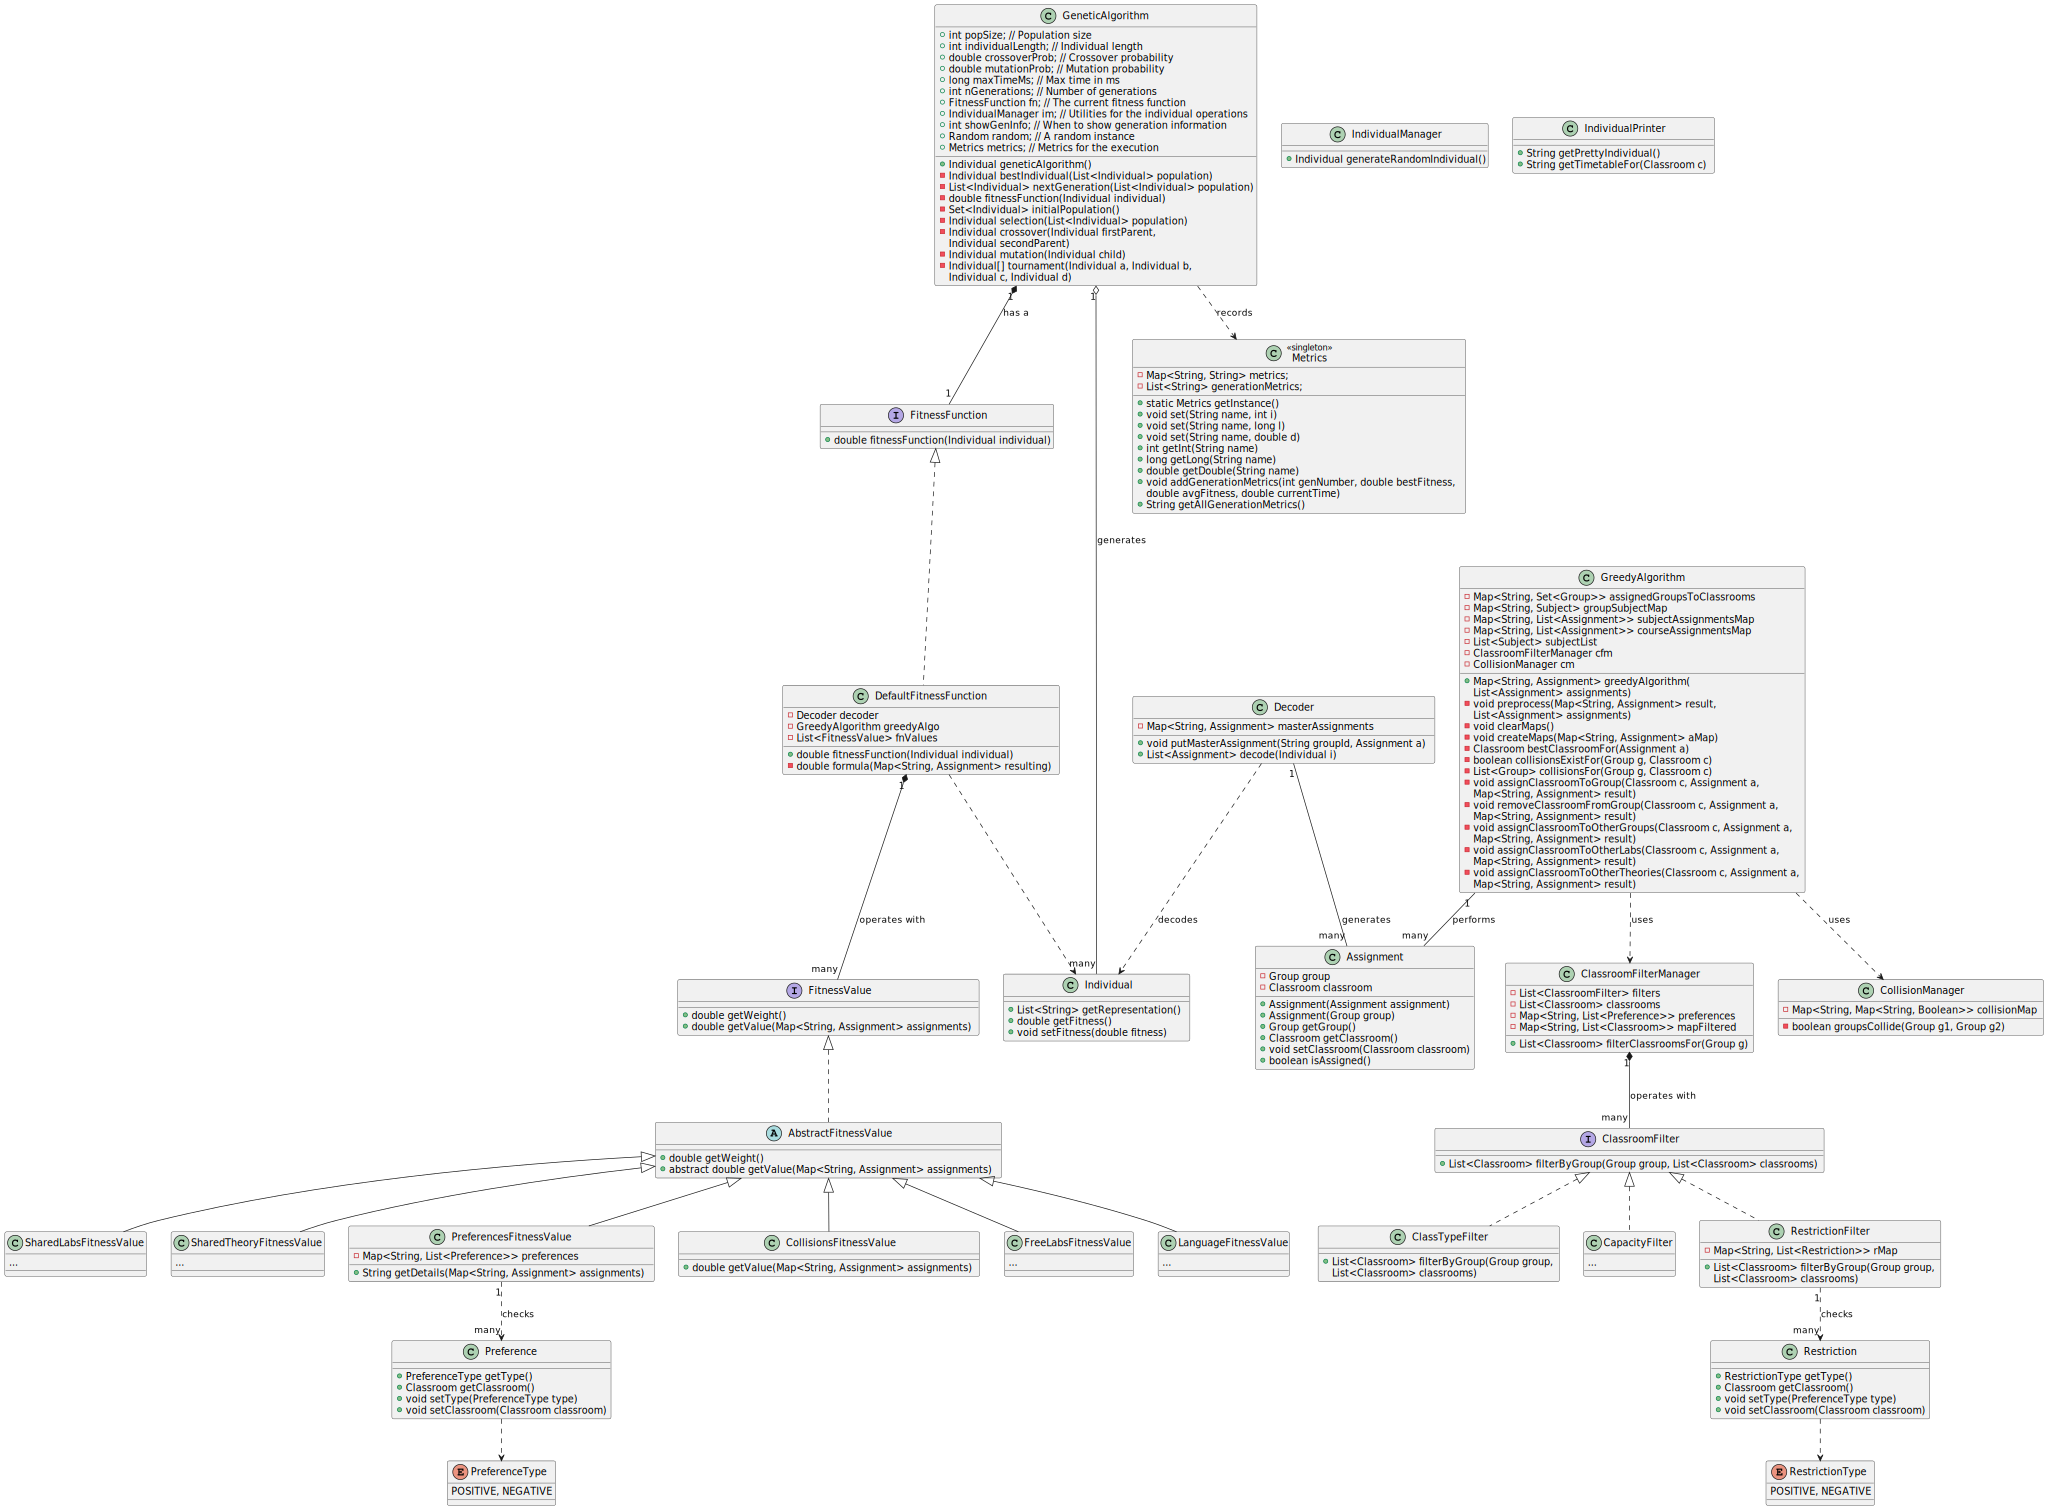
\includegraphics[scale=0.15]{final_alg_class_diagram_uml.png}
\end{figure}

\begin{figure}[H]
    \caption{Class diagram: Alg package (Greedy algorithm)}
  \centering
  \includegraphics[scale=0.28]{final_alg_greedy_class_diagram_uml.png}
\end{figure}

\begin{figure}[H]
    \caption{Class diagram: Alg package (Genetic algorithm)}
  \centering
  \includegraphics[scale=0.27]{final_alg_genetic_class_diagram_uml.png}
\end{figure}

\begin{figure}[H]
    \caption{Class diagram: Problem domain}
  \centering
  \includegraphics[scale=0.35]{final_problem_class_diagram_uml.png}
\end{figure}

\begin{figure}[H]
    \caption{Class diagram: Other business classes}
  \centering
  \includegraphics[scale=0.28]{final_business_other_class_diagram_uml.png}
\end{figure}

\begin{figure}[H]
    \caption{Class diagram: Persistence}
  \centering
  \includegraphics[scale=0.24]{final_persistence_class_diagram_uml.png}
\end{figure}



\section{Interaction and state diagrams}

\section{Activity diagram}

\section{Interface design}

\section{Technical specification of the test plan}

 

    \newpage
    \renewcommand{\documentname}{System implementation}

\chapter{System implementation}


\section{License and references}

\subsection{License}

The software of this project is licensed under the GNU General Public License v2.0.

\subsection{References}

\begin{itemize}
    \item \textit{Java Code Conventions.} Set of guidelines and conventions for programmers to consider when using the Java programming language.

    \item \textit{Linux kernel coding style.} \footnote{Available at \url{https://www.kernel.org/doc/Documentation/process/coding-style.rst}} Set of guidelines and conventions for programmers to consider when programming in the Linux kernel. The stylistic choices in this guide have, for the most part, been the ones adopted for formatting the prototype code, as we believe that the readability of the code is preferable to the Java Code Conventions guidelines.
\end{itemize}



\section{Programming languages}

The use of C or Java for programming the system was discussed. In the end we opted for Java for two reasons. The first is simple, I, the developer, have more experience in Java than in C (although I have used both in this School). Perhaps C would be a suitable language to implement the algorithms described in this document more efficiently, but the extra time I would have to spend learning the language in an advanced way makes it unmanageable for this project. The second reason is also obvious. If this project is to be continued by our colleagues at the School, it would be preferable if it were written in the language that has been learnt throughout the degree courses, i.e, Java.

\section{Tools and programs used in development}

\section{System development}

 

    \newpage
    \renewcommand{\documentname}{Test development}

\chapter{Test development}

 

    \newpage
    \renewcommand{\documentname}{Experimental results}

\chapter{Experimental results}\label{experimental-results}

This chapter shows the various experimental studies carried out to evaluate the quality of the prototype and its algorithms. We advance the main thesis we have arrived at after this study: The greedy algorithm is able to solve the problem without the help of the genetic algorithm. However, it is not powerful enough to find the best solutions obtained with other configurations. Only when coupled with the best version of the genetic algorithm does the software perform at its best.


\subsection{Instances}

Four scenarios have been identified for this phase. One scenario is a combination of a group loading level and a constraint loading level. We have groups from the first and second semester of two different academic years, and we have restrictions and preferences obtained from client meetings.

For the charged load level, one group per subject was created for each instance with a 10\% probability, and one restriction or preference with a 20\% probability. Once created, the results were checked for incorrect data or contradictions.

We therefore have the following scenarios:

\begin{itemize}
    \item \textbf{Charged groups - Charged constraints}
    \item \textbf{Charged groups - Regular constraints}
    \item \textbf{Regular groups - Charged constraints}
    \item \textbf{Regular groups - Regular constraints}
\end{itemize}


\subsection{Initial fitness function}

The initial fitness function is created based on the client's expectations of results. The highest weight is given to all assignments being performed, followed by the fulfilment of preferences, then the remaining fitness values.

The values for the initial fitness function follow.

\begin{lstlisting}[basicstyle=\small]
# Fitness weights

# COL_WEIGHT: Weight for the collisions fitness value
COL_WEIGHT = 1.0

# FREE_LABS_WEIGHT: Weight for the free labs fitness value
FREE_LABS_WEIGHT = 0.25

# LANG_WEIGHT: Weight for the group language fitness value
LANG_WEIGHT = 0.25

# SHARED_LABS_WEIGHT: Weight for the shared labs fitness value
SHARED_LABS_WEIGHT = 0.25

# SHARED_THEORY_WEIGHT: Weight for the shared theory classes fitness value
SHARED_THEORY_WEIGHT = 0.25

# PREFS_WEIGHT: Weight for the preferences fitness value
PREFS_WEIGHT = 0.5
\end{lstlisting}



\subsection{Greedy Algorithm reviews}

With this initial fitness function, we proceed to experiment with the following versions of the greedy algorithm:

\begin{itemize}
    \item \textbf{Base greedy}: Algorithm without repairs and biases.
    \item \textbf{Base greedy + Repairs}: Algorithm with repairs but without biases.
    \item \textbf{Base greedy + Repairs + Biases}: Algorithm with repairs and biases towards preferences and shared classrooms.
\end{itemize}


\subsubsection{Fitness reviews}

\subsubsection{Metric reviews}


\subsection{(Genetic + Greedy) parameter reviews}

\subsection{Further fitness functions}

 

    \newpage
    \renewcommand{\documentname}{System manuals}

\chapter{System manuals}


\section{Installation manual}

\section{Execution manual}

\section{User manual}

\section{Programmer manual}

 

    \newpage
    \renewcommand{\documentname}{Conclusions and future work}

\chapter{Conclusions and future work}

\section{Final conclusions}

All the objectives set for the project have been met. A study and formalisation of the problem has been carried out and the problem was solved, both theoretically and experimentally, thanks to a software tool that was developed in this project.

The files necessary for the software to work have been designed and created. They are provided in the annexes, many of which can be reused by the user of the application. In addition, an experimental study has been conducted on the developed solution in order to provide the customer with the default configuration of the system to ensure quality results in various possible scenarios.

The developed system is licensed under a free software licence and may be modified and distributed by users who wish to do so.

With all this in mind, the project comes to a close with satisfaction on my part, although the work does not end here. In the next section, some possible lines for the continuation of the work developed in this project are explained.


\section{Future work}

Although the objectives of the project have been met, nothing changes the fact that the software designed in this document is a prototype. Of course, a fully usable prototype with interesting functionalities, but there is room for improvement. Listed below are some lines of research and development to be pursued on the basis of this project.


\begin{itemize}
    \item \textbf{Expansion of the class search functionality to return results that support multiple events}. Currently the user can browse the results looking for free classes at the same time, but perhaps it would be useful to have a feature that allows the users to choose the number of classes they are seeking for an event that are available at the same time.
    \item \textbf{Increased validation of input files}. The current validation is perfectly valid, and can help the user to find most of the problems. However, more specific checks such as the formatting of a group/class/subject code, that the end dates of queries are not less than the start dates, etc, would provide a better user experience.
    \item \textbf{Possibility of assigning different classes to each group depending on the day}. This is \textit{very complicated}, as it affects the main pillar of the whole theory that a group can only have one classroom associated with it. However, if one wanted to rethink the problem from scratch, this approach could be taken into account. Hopefully, such an approach would serve to further reduce the number of unassigned groups.
    \item \textbf{Rewrite the code in a language such as C or Go, more focused on algorithms}. It should be noted that the code described here, as mentioned above, is only a prototype. It can and does work correctly, but if new functionalities appear that greatly affect the original design, one should not be afraid to rewrite the code, and in that case, another language could be used. Shorter computation times could be expected if the system is implemented in this kind of languages.
\end{itemize}


 

    \newpage
    \renewcommand{\documentname}{Budget}

\chapter{Budget}

\section{TODO}

TODO

 

    \newpage
    \renewcommand{\documentname}{Annexes}

\chapter{Annexes}


\section{Definitions and abbreviations}

Listed below is a glossary of definitions and abbreviations used in the document whose meaning may not be obvious.

Glossary of definitions:

\begin{itemize}
    \item \textbf{Genetic algorithm:} metaheuristic search and optimization algorithm. 
    \item \textbf{Greedy algorithm:} algorithm that builds the solution in successive steps, always trying to take the optimal solution for each step
    \item \textbf{Heuristic:} function that gives value to each path in a search algorithm, based on current information.
    \item \textbf{Java:} general-purpose, high-level, object-oriented programming language.
    \item \textbf{Metaheuristic:} high-level heuristic that guides the search in a combinatorial optimization problem.
\end{itemize}

Glossary of abbreviations:

\begin{itemize}
    \item \textbf{CSV:} Comma-Separated Values. Refers to a text file format.
    \item \textbf{CLI:} Command Line Interface.
    \item \textbf{GNU:} GNU is not Unix (recursive acronym). Refers to the free software project announced by Richard Stallman.
    \item \textbf{TXT:} Text. Refers to the text file format.
    \item \textbf{UNE:} in spanish, \textit{Una Norma Española}. Refers to the Spanish Association for Standardisation.
\end{itemize}


\section{Submission contents}

 

    \newpage
    \renewcommand{\documentname}{Source code}

\chapter{Source code}

 

    \newpage
    \renewcommand{\documentname}{Bibliography}

\chapter{Bibliography}

\section{TODO}

TODO



}

\renewcommand{\documentname}{Bibliography}

\end{document}

